% Author :  Lionel du Peloux
% Contact : lionel.dupeloux@gmail
% Year : 2017
% !TEX encoding = UTF-8 Unicode

\newrefsegment
\chapter{Numerical Model}\label{chp=numerical_model}

\section{Introduction}
In this chapter we construct a novel discrete beam element that we call the \emph{biarc beam element}. It relies on the results from \cref{chp=curve} and \cref{chp=kirchhoff}.

This element has a minimal number of degrees of freedom due to a reduced discrete curve-angle representation and can model extension, flexion and torsion of the rod in the framework of Kirchhoff theory. The introduction of ghost vertices enriches our previous model \cite{DuPeloux2015,Lefevre2017} in order to better represent and localize discontinuities in the model. In particular this leads to a more accurate treatment of boundary conditions, connections and loadings. This element easily integrates inside a Dynamic Relaxation (DR) procedure to find the static equilibrium of nonlinear problems.

In the end, that makes this element very suitable for the modeling of elastic gridshells with anisotropic cross-sections and complex connections, which are known limitations of the classical \dofs{3} spline beam element \cite{Adriaenssens2001,Douthe2006}. Moreover, the reduced formulation should improve both speed and stability of the numerical method compared to the classical \dofs{6} beam element \cite{Adriaenssens2000,DAmico2014}.

The interest of our approach is that the entire model is derived directly from the motion equations of the rod and thus is perfectly in the line of the pioneer works in this field \cite{Day1965}.

\subsection{Overview}
We first construct a novel discrete beam element called the \emph{biarc model} (see \cref{sec=dmodel}). This element is based on Kirchhoff theory of slender rods presented in \cref{chp=kirchhoff}. The mechanical behavior of the element is derived entirely from the equations of motion \cref{eq:motion} summarized in \cref{sec=ksummary}~:
\begin{itemize}
\item we compute the discrete force ($\vect{\eta}$) and moment ($\vect{\varkappa}$) strain vectors from the geometry of the centerline~;
\item we compute the bending moment ($\vect{M}^{\perp}$) at vertices from the material constitutive laws~;
\item we compute the twisting moment ($\vect{Q}$) and the axial force ($\vect{N}$) at mid-edges from the material constitutive laws~;
\item we compute the shear force ($\vect{F}^{\perp}$) at mid-edges from the equations of motion \cref{eq:motion_4,eq:motion_5}~;
\item we interpolate the twisting moment and the axial and shear forces at vertices~;
\end{itemize}
Once the internal forces and moments acting on the vertices of the rod are known, we reinterpret the rod model as a simple \emph{particle-spring} system (see \cref{sec=DR}). We study the motion of this system by integrating explicitly the motion equations of the particles with a simple finite difference scheme. The motion is artificially damped so the system falls into a state of static equilibrium. This method is called the \emph{Dynamic Relaxation}. The dynamic itself is not a matter of concern as we are only interested in the steady state. Therefore, the parameters of the dynamic (mass and time step) are optimized to achieve \emph{critical damping}, the damping for which the convergence is the fastest, and to ensure the numerical stability of the method.

Boundary conditions and connections between rods are treated separately (see \cref{sec=enriching}). This topic is of special interest when modeling real structures, which is our ultimate goal.

The model has been implemented in a C\# library called \emph{Marsupilami}, intended to be a lightweight and dependence-free portable API. It is not a standalone executable software and has no graphical user-interface (GUI). To that purpose, a plugin for \grasshopper{} has also been implemented which serves as a functional GUI inside the \rhino{} environnement. The core concepts of \emph{Marsupilami} are presented in \cref{sec=software}. This work was the occasion to develop a finer understanding of software architecture. Several guidelines are proposed to further develop what is more a prototype and validation code than a full-featured software.

Finally, several test cases are presented to validate the model (see \cref{sec=testcase}).

\subsection{Contributions}
\begin{itemize}
	\item We introduce a new \dofs{4} biarc kinematic to model the rod motion with ghost and handle vertices.
	\item We clarify the representation of edge and vertex quantities in a natural manner where material and cross-section properties are associated to the edges, and internal forces and moments are associated to the vertices.
	\item The biarc kinematic allows to model discontinuities at the junction between biarc segments.
	\item The mechanic of the rod is entirely derived from the motion equations.
	\item We give a full treatment of boundary conditions.
	\item We implement our element inside a Dynamic Relaxation algorithm.
	\item We use parallel transport only locally so that there is no more need to maintain a global reference frame for each beam.
\end{itemize}

\subsection{Related works}

\subsubsection{Dynamic Relaxation}

\citef{Day1965} introduces the \emph{Dynamic Relaxation} method also presented by \citef{Otter1966}. He remarks that for a damped system the \blockquote{static equilibrium of a structure under a system of applied forces may be found by following the movement of the structure from its initial, un-deformed and unloaded, position until all vibrations resulting from its subsequent loading have died out}. He proposes to choose the damping factor to achieve critical damping, that is to obtained the fastest convergence to the steady state. He uses this computing method to study the non linear deformation of planar portal frames parameterized by two rotational degrees of freedom.

\citef{Cassel1976} study the stability of the method. They formulate a stability criterion expressed as a relation between the time step, the mass and the entries of the stiffness matrix. A similar criterion is formulated by \citef{Barnes1975}. Later, a proof of this criterion using Gershgorin theorem is made by \citef{Papadrakakis1981} and \citef{Underwood1983} who achieved automatic determination of the Dynamic Relaxation parameters to ensure stability but not necessarily critical damping.

\citef{Barnes1977} uses the Dynamic Relaxation to design and analyze nonlinear cable, membrane and inflatable structures. \citef{Wakefield1980} uses Dynamic Relaxation to study pretension networks with compression arches. He remarks that the method can be interpreted as a first order gradient optimization method. He first introduces a simplified planar bending element \cite[p.~120]{Wakefield1980}, which is the parent of the classical \dofs{3} spline beam element. A review of the work from Barnes, Wakefield and Papadrakakis is available in \cite{Barnes1999}.\footnote{Wakefield and Papadrakakis where phd students of Barnes in the late 70's.}

Interesting investigations of the use of Dynamic Relaxation are proposed by \cite{Rodriguez2011a} for the study of inflatable structures and by \citef{Dang2010} for geotechnical engineering. \citef{Silva2006} show the efficiency of the Dynamic Relaxation method compared to the Newton-Rapshon method in the nonlinear simulation of flexible lines. He highlights the robustness of the Dynamic Relaxation method, able to reach convergence where the Newton-Rapshon method fails.

\citef{Rezaiee2012} propose a very large scope benchmark of Dynamic Relaxation method variants. His results show that the kinetic damping variant \cite{Topping2007} has generally the fastest convergence CPU speed, while the viscous damping variant from Underwood \cite{Underwood1983} generally converges with the smallest number of iterations.

\citef{Miki2014} also interpret Dynamic Relaxation as a gradient descent method. They extend the method to integrate equality constraint conditions. However, the proposed method does not exhibit a better convergence speed than the one with kinetic damping.

Bathe is a reference author in the field of structural dynamics. He has worked on many time integration methods, either implicit or explicit \cite{Noh2013}. His work could be a valuable starting point to pick new ideas to improve the time integration scheme presented in this thesis, if the dynamic of the structure were to be studied for instance.

\subsubsection{Discrete element}

The classical \dofs{3} spline beam element is formulated by Adriaenssens, Barnes, and Williams \cite{Barnes1999,Adriaenssens1999,Adriaenssens2001}. This model is used by \citef{Douthe2006} for the form-finding of elastic gridshells in composite materials. They improve the calculation of the lumped mass to take account for the geometric bending stiffness of the element. They formulate a connection model that takes into account the eccentricity between the structural members.

\citef{Adriaenssens2000} introduces a \dofs{6} beam element compatible with the Dynamic Relaxation method. This element is implemented by \citef{Olsson2012}, \citef{Poulsen2015} and \citef{DAmico2014} in custom numerical frameworks to study nonlinear behavior of grid structures.

A first attempt to formulate a reduced model that takes into account torsion in the element is made by \citef{Barnes2013}. Twisting is evaluated by the measure of the geometric torsion of the centerline, which obviously gives correct results in very special cases. Following \citef{Bergou2008}, Tayeb, Lefevre and du Peloux propose a novel \dofs{4} beam element suitable for the structural analysis of elastic gridshells \cite{DuPeloux2015,Lefevre2017}. A closely related work is proposed by \citef{DAmico2016} but relies on a Catmull-Rom spline interpolation that complexifies the treatment of the element end nodes.

\citef{Duan2013} develop a geometrically exact beam model with a finite-element formulation to capture dynamic elastic deformations of slender bodies. The ordinary differential equations are solved using a multiple shooting algorithm based on numerical integration with Runge–Kutta method. Although the results show a good accuracy, the computational cost seems prohibitive for real-time rendering of grid structures with a large number of connections.





%Pour des cas test :
%\citef{Ibrahimbegovic1995}

\section{Discret beam element}\label{sec=dmodel}
% =======================
Let us introduce the discrete \emph{biarc} model to describe the configuration of a beam. It is composed of a discrete curve called \emph{centerline} ($\Gamma$) and a discrete adapted frame called \emph{material frame} as its axes are chosen to be the principal axes of the beam cross-section (\cref{fig:discrete_model}). The centerline itself is organized in $n_s$ consecutive adjacent \emph{segments} which are three-vertices and two-edges elements with uniform material and section properties.

Elements can either be closed or open. The relations between the corresponding number of vertices, edges and segments are reported in \cref{tab:count}.

\begin{figure}[p]
\begin{fullpage}
	\captionsetup[subfloat]{captionskip=20pt}
     	\centering
     	\subfloat[][Centerline of the discrete biarc model]{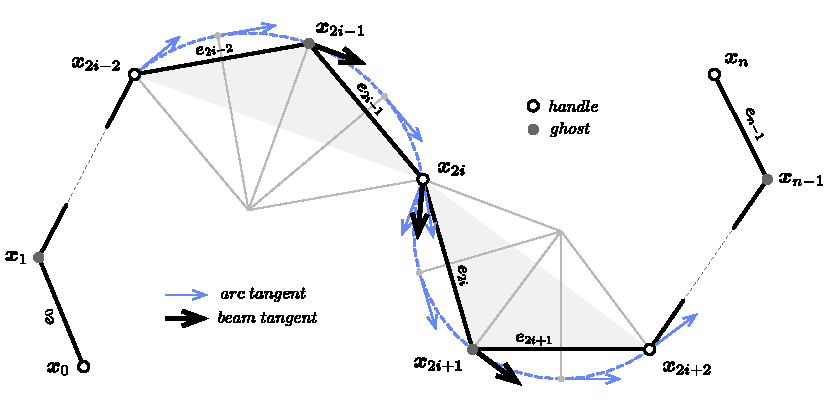
\includegraphics{discrete_model.pdf}\label{fig:discrete_model}} \\
	\vspace{30pt}
	\subfloat[][Number of segments, edges and vertices whether the centerline is closed or open]{\label{tab:count}%
		 \ra{1.2}
		 \begin{tabularx}{0.45\textwidth}{@{} X l r  r@{}}
		 \toprule
		 		&			& \multicolumn{2}{c}{Centerline} \\ \cmidrule(l){3-4}
		 Item 	&  Symbol 	& Open 	& Closed \\
		 \midrule
		segments & $n_s$ & $n_s$ & $n_s$ \\
		edges & $n_e$ & $2 n_s$ & $2 n_s$ \\
		vertices & $n$ & $2 n_s + 1$ & $2 n_s$ \\
		ghosts & $n_g$ & $n_s$ & $n_s$ \\
		handles & $n_h$ & $n_s+1$ & $n_s$ \\
		\bottomrule
		
	\end{tabularx}}
	\vspace{10pt}
	\captionof{figure}[Biarc model for a discrete beam element]{Biarc model for a discrete beam element. The centerline is divided into curved segments (grey solid hatch). Each segment is defined as a three-noded element with uniform material and section properties. It has two end vertices (white) called \emph{handle} as they are used to interact with the model, for instance to apply loads or restrains. It has one mid vertex (grey) called \emph{ghost} as it is used only to enrich the segment kinematics and is not accessible to the end user.}
\end{fullpage}
\end{figure}

\subsection{Description of the element}
Here we present how we model all the required informations involved in the element representation~: its geometry (centerline, material frames, cross-sections), its materiality (elastic and shear modulus) and its mechanical state (internal forces and moments). An element is also subject to external loads (external forces and moments).
\subsubsection{Centerline}
% --------------------------------
The discrete centerline is a polygonal space curve (\cref{fig:discrete_model}) defined as an ordered sequence of $n+1$ pairwise disjoint \emph{vertices}~: $\Gamma = (\vect{x}_0,  \vect{x}_1, \ldots, \vect{x}_n) \in \mathbb{R}^{3(n+1)}$. Consecutive pairs of vertices define $n$ straight segments $(\vect{e}_0,  \vect{e}_1, \ldots, \vect{e}_{n-1})$ called \emph{edges} and pointing from one vertex to the next one~:
\begin{subequations}
	\begin{alignat}{1}
	\vect{e}_i 	&= \vect{x}_{i+1} - \vect{x}_{i}
	\\
	l_i 		&= \norm{\vect{e}_i}
	\\
	\vect{u}_i 	&= \vect{e}_i / l_i = \vect{d}_{3, i+1/2}
	\end{alignat}
\end{subequations}
The length of the $i$th edge is denoted $l_i $ and its normalized direction vector is denoted $\vect{u}_i$. The arc length of the $i$th vertex is denoted $s_i$ and is given by~:
\begin{equation}
	\left\{
	\begin{aligned}
		s_0 	&= 0 				& 	&i = 0		\\
		s_i 	&= \sum_{k=0}^{i-1} l_k	&	&i \in \llbracket 1, n-1 \rrbracket	\\
		s_n 	&=  L 				&	&i = n		\\
	\end{aligned}
	\right.
\end{equation}
Thus, the centerline is parameterized by arc length and $\Gamma(s_i) = \vect{x}_i$. Additionally, we define the vertex-based mean length at vertex $\vect{x}_i$~:
\begin{equation}
%\setlength{\jot}{8pt}
	\left\{
	\begin{aligned}
		\rconf{l}_0 	& =  \tfrac{1}{2}l_0				&		&i = 0					\\
		\rconf{l}_i	& =  \tfrac{1}{2}(l_{i-1} + l_i)		&		&i \in \llbracket 1, n-1 \rrbracket	\\
		\rconf{l}_n 	& =  \tfrac{1}{2}l_{n-1} 			&		&i = n					\\
	\end{aligned}
	\right.
\end{equation}

\subsubsection{Segments}
% ---------------------------------
The discrete centerline is divided into $n_s$ curved segments. Each segment is a three-noded element where the area covered by a segment is represented as a grey solid hatch (see \cref{fig:discrete_model}). The $i$th segment is composed of three vertices ($\vect{x}_{2i}, \vect{x}_{2i+1},  \vect{x}_{2i+2}$) spanning two edges ($\vect{e}_{2i}, \vect{e}_{2i+1}$). The ($i-1$)th segment and the $i$th segment share the same vertex $\vect{x}_{2i}$ at arc length $s_{2i}$.

Each segment has two end vertices called \emph{handle} ($\vect{x}_{2i}, \vect{x}_{2i+2}$) and one mid vertex called \emph{ghost} ($\vect{x}_{2i+1}$) as this one is not accessible to the end user in order to interact with the model (link, restrain, loading, \dots). Ghost vertices are used only for internal purpose to give a higher richness in the kinematic description of a segment than a two-noded segment would.

Finally, we define the \emph{chord length} of the $i$th segment as the distance between $\vect{x}_{2i}$ and $\vect{x}_{2i+2}$~:
\begin{equation}
	L_i = \norm{\vect{e}_{2i} + \vect{e}_{2i+1}} \quad , \quad i \in \llbracket 0, n_s-1 \rrbracket
\end{equation}

\subsubsection{Material frames}
% ---------------------------------------
A discrete material frame $\{\vect{d}_{1}, \vect{d}_{2}, \vect{d}_{3}\}_i$ is associated to each vertex $\vect{x}_i$. Material directors $\vect{d}_{1,\,i}$ and $\vect{d}_{2,\,i}$ are chosen to be aligned with the principle axes of the cross-section at vertex $\vect{x}_i$. At mid edge, the definition of $\vect{d}_{3,\,i+1/2}$ is consistent with the discrete curvature based on the circumscribed osculating circle (see \cref{sec=discrete_tangent_circumscribed}).

\subsubsection{Material and section properties}
% ------------------------------------------------------------
In addition, the model assumes that a segment has uniform section ($S$, $I_1$, $I_2$, $J$)\footnote{$S$ is the cross-section area ; $I_1$, $I_2$ and $J$ are the principal moments of inertia of the cross-section.} and material ($E$, $G$)\footnote{$E$ is the elastic modulus and $G$ is the shear  modulus for the considered material.} properties over its length $s \in ]s_{2i},s_{2i+2}[$. For the sake of simplicity, we introduce for further calculations the \emph{material stiffness matrix} ($\mat{B}_i$) attached to each segment. It has the following form in the material frame basis~:
\begin{equation}
	\mat{B}_i = \begin{bmatrix}
			EI_1		&	0		&	0		\\
			0		&	EI_{2}	&	0		\\
			0		&	0		&	GJ_{}	\\
		\end{bmatrix}_i
	\quad , \quad i \in \llbracket 0, n_s-1 \rrbracket
	\label{eq:stiffnessmatrix}
\end{equation}
where $EI_1$ and $EI_2$ are the bending stiffnesses and $GJ$ is the torsional stiffness. The axial stiffness of the $i$th segment is denoted by :
\begin{equation}
	ES_i 	\quad , \quad i \in \llbracket 0, n_s-1 \rrbracket
\end{equation}

 \subsubsection{Internal forces and moments}
% ---------------------------------------------------------
The discrete rod is subjected to internal forces ($\vect{F} = F_1 \vect{d}_1 + F_2 \vect{d}_2 + \vect{N}\vect{d}_3$) and moments ($\vect{M} = M_1 \vect{d}_1 + M_2 \vect{d}_2 + Q\vect{d}_3$). Their components in the material frame basis are named as follow :
\begin{itemize}
\item The shear force : $\vect{F}^{\perp} = F_1 \vect{d}_1 + F_2 \vect{d}_2$
\item The axial force : $\vect{N} = N \vect{d}_3$
\item The bending moment : $\vect{M}^{\perp} = M_1 \vect{d}_1 + M_2 \vect{d}_2$
\item The twisting moment : $\vect{Q} = Q \vect{d}_3$
\end{itemize}

\subsubsection{Distributed loads}
% -----------------------------------------
The model assumes that each segment can be loaded with some distributed forces ($\vect{f}^{ext} = f_k\vect{d}_k$) and moments ($\vect{m}^{ext} = m_k\vect{d}_k$). These forces and moments are required to be uniform over each segment but can vary from one segment to another. They can represent body loads such as self weight or thermal loads~; or external loads such as wind, snow, pressure,~\dots

\subsubsection{Concentrated loads}
% ---------------------------------------
Additional external concentrated forces ($\vect{F}^{ext}$) and moments ($\vect{M}^{ext}$) are applied to the segment's end vertices ($\vect{x}_{2i}$,  $\vect{x}_{2i+2}$). Note that the model does not allow to load ghost vertices, and this is precisely why they are called \emph{ghost}.

% Modeling discontinuities
% ------------------------------------
 \subsection{Modeling of discontinuities}
The model assumes that cross-section and material properties as well as distributed loads are uniform over each segment. Referring to the structure of the equations of motion, and because the centerline is required to be a regular curve in the stress-free configuration, strains, stresses, displacements, internal forces and internal moments must be piecewise continuous functions of the arc length parameter, continuous over each segment $]s_{2i},s_{2i+2}[$. Discontinuities of these functions might occur at handle vertices ($\vect{x}_{2i}$), for instance if there is a jump in material or cross-section properties or if concentrated loads are applied at handle vertices. Moreover, the centerline curve itself will stay $\mathcal{C}^1$ during the motion, as it is chosen to be $\mathcal{C}^1$ in the reference configuration.\footnote{This preclude the modeling of beams with kinks as the tangent vector would not be continuously defined at these points. In such a case, the beam should be modeled in two separate parts linked together in a rigid manner.}\textsuperscript{,}\footnote{The centerline is not necessarily $\mathcal{C}^2$ as discontinuities in curvature may occur. For instance, if no punctual loads are applied, the bending moment is continuous over the rod. As the bending moment is linked to the curvature through the constitutive equation $M = EI\varkappa$, a discontinuity in $I$ will lead to a discontinuity in $\varkappa$. Conversely, a discontinuity in $\varkappa$ will lead to a discontinuity in $I$.}

Here and subsequently, for such a function the left and right limits at handle vertices ($s_{2i}$) will be denoted with superscripts $f_{2i}^-$ and $f_{2i}^+$. Possibly, the function is continuous so that the left and right limits agree ($f_{2i}^- = f_{2i}^+$).

% Matrix notation
% --------------------
\subsection{Matrix notation}
Here and subsequently, matrix notation will often be used to provide compact expressions for the equations, where the components of vector-valued functions are given in the material frame basis. This notation will be mixed with the vector notation employed  more generally throughout this document. Usually, if there is no comment in the manuscript, the meaning should be obvious and with no ambiguity to the reader.

For instance, all this expressions for the curvature binormal vector and the material curvatures vector will be considered equivalent and could be mixed together in the same equation~:
\begin{subequations}
	\begin{alignat}{1}
	&\vect{\kappa b}
	= \kappa_1 \vect{d}_1 +  \kappa_2 \vect{d}_2
	= \begin{bmatrix} \kappa_1 & \kappa_2 & 0 \end{bmatrix}^T
	\\
	&\vect{\varkappa}
	= \varkappa_1 \vect{d}_1 +  \varkappa_2 \vect{d}_2 +  \varkappa_3 \vect{d}_3
	= \begin{bmatrix} \varkappa_1 & \varkappa_2 & \varkappa_3 \end{bmatrix}^T
	= (1+\epsilon) \begin{bmatrix} \kappa_1 & \kappa_2 & \tau \end{bmatrix}^T
	\end{alignat}
\end{subequations}
The force strains vector is given by :
\begin{equation}
	\vect{\eta} = (1+\epsilon)\vect{d}_3 = \begin{bmatrix} 0 & 0 & 1+\epsilon \end{bmatrix}^T
\end{equation}
Internal forces are composed of a shear force and an axial force given by~:
\begin{subequations}
	\begin{alignat}{3}
	&\vect{F}
	&&= F_1 \vect{d}_1 +  F_2 \vect{d}_2 + N \vect{d}_3
	= \begin{bmatrix} F_1 & F_2 & N \end{bmatrix}^T
	\\
	&\vect{F}^{\perp}
	&&= F_1 \vect{d}_1 +  F_2 \vect{d}_2
	= \begin{bmatrix} F_1 & F_2 & 0 \end{bmatrix}^T
	\\
	&\vect{F}^{\para} &&= \vect{N}
	= N \vect{d}_3
	= \begin{bmatrix} 0 & 0 & N \end{bmatrix}^T
	\end{alignat}
\end{subequations}
Internal moments are composed of a bending moment and a twisting moment given by~:
\begin{subequations}
	\begin{alignat}{3}
	&\vect{M}
	&&= M_1 \vect{d}_1 +  M_2 \vect{d}_2 + Q \vect{d}_3
	= \begin{bmatrix} M_1 & M_2 & Q \end{bmatrix}^T
	\\
	&\vect{M}^{\perp}
	&&= M_1 \vect{d}_1 +  M_2 \vect{d}_2
	= \begin{bmatrix} M_1 & M_2 & 0 \end{bmatrix}^T
	\\
	&\vect{M}^{\para} &&= \vect{Q}
	= Q \vect{d}_3
	= \begin{bmatrix} 0 & 0 & Q \end{bmatrix}^T
	\end{alignat}
\end{subequations}
With the help of the matrix notation, the constitutive equations \cref{eq:constitutive_b,eq:constitutive_c,eq:constitutive_d} together write in a single equation~:
\begin{equation}
	\mat{M} = \mat{B} (\vect{\varkappa} - \rconf{\vect{\varkappa}})
	= EI_1(\varkappa_1 - \rconf{\varkappa}_1) \vect{d}_1
	+ EI_2(\varkappa_2 - \rconf{\varkappa}_2) \vect{d}_2
	+ GJ (\varkappa_3 - \rconf{\varkappa}_3) \vect{d}_3
\end{equation}

%We also introduce the matrix notation for the derivatives of the internal forces and moments referring to the inertial frame of reference $\{\vect{x},\vect{y},\vect{z}\}$ and to the local frame $\{\vect{d}_{1},\vect{d}_{2},\vect{d}_{3}\}$. The (spatial) velocity of $\{\vect{d}_{1},\vect{d}_{2},\vect{d}_{3}\}$ implies that~:
%\begin{subequations}
%	\begin{alignat}{3}
%	&\vect{F}' = \vect{F}^{'|xyz} = \vect{F}^{'|123} + \vect{\varkappa} \times \vect{F}
%	\\
%	&\vect{M}' = \vect{M}^{'|xyz} = \vect{M}^{'|123} + \vect{\varkappa} \times \vect{M}
%	\end{alignat}
%\end{subequations}
%where $\vect{F}_{xyz}'$ and $\vect{M}_{xyz}'$ denote the derivative with respect to $s$ in the inertial frame of reference $\{\vect{x},\vect{x},\vect{z}\}$ whereas $\vect{F}_{123}'$ and $\vect{M}_{123}'$ denote the derivative with respect to $s$ in the local material frame basis $\{\vect{d}_{1},\vect{d}_{2},\vect{d}_{3}\}$. Thus the matrix notation for $\vect{F}_{123}'$ and $\vect{M}_{123}'$ are given by :
%\begin{subequations}
%	\begin{alignat}{3}
%	&\vect{F}^{'|123}
%	&&= F_1' \vect{d}_1 +  F_2' \vect{d}_2 + N' \vect{d}_3
%	= \begin{bmatrix} F_1' & F_2' & N' \end{bmatrix}^T
%	\\
%	&\vect{M}^{'|123}
%	&&= M_1' \vect{d}_1 +  M_2' \vect{d}_2 + Q' \vect{d}_3
%	= \begin{bmatrix} M_1' & M_2' & Q' \end{bmatrix}^T
%	\end{alignat}
%\end{subequations}

% Discret extension and axial force
% --------------------------------------------
\subsection{Discret extension and axial force}
We assume the axial force ($\vect{N}$) to vary linearly over $]\vect{x}_{2i},  \vect{x}_{2i+2}[$ with the arc length parameter. The variation occurs if the segment is subject to a uniform distributed load $f_3$ over the segment. Consequently, the axial strain $\epsilon$ is also required to vary linearly. The value of the axial extension at mid span of each edge is given by~:
\begin{equation}
	\epsilon_{i+1/2} = {l_{i}}\,/\,{\rconf{l}_i} - 1 \quad , \quad i \in \llbracket 0, n_e-1 \rrbracket
\end{equation}
Consequently, the axial force at mid span of each edge is computed directly with the constitutive equation \cref{eq:constitutive_a} as~:
\begin{subequations}
	\begin{alignat}{3}
	\vect{N}_{2i+1/2} &= N_{2i+1/2}\, \vect{u}_{2i} \quad &&\text{where} \quad {N_{2i+1/2}} = ES_i \,\epsilon_{2i+1/2}
	\\
	\vect{N}_{2i+3/2} &= N_{2i+3/2}\, \vect{u}_{2i+1}\quad &&\text{where} \quad {N_{2i+3/2}} = ES_i \,\epsilon_{2i+3/2}
	\end{alignat}
\end{subequations}
Remark the sign convention~: as expected, when edge $\vect{e}_i$ suffers a positive extension ($\epsilon_{i+1/2} > 0$), vertex $\vect{x}_{i+1}$ \textquote{attracts} vertex $\vect{x}_{i}$ to it as $\vect{d}_{3,i+1/2} = \vect{u}_{i}$ is pointing from $\vect{x}_{i}$ towards $\vect{x}_{i+1}$. Remark also that $\epsilon_{i+1/2} = 0 \Leftrightarrow l_i = \rconf{l}_i$ when the rod is not stretched.

% Discret bending moments and curvatures
% -------------------------------------------------------
\subsection{Discret curvature and bending moment}
We assume that the internal bending moment and curvature are quadratic functions of the arc length parameter over $]\vect{x}_{2i},  \vect{x}_{2i+2}[$.
Although they must be continuous over this interval, they might be discontinuous at handle vertices and be subjected to jump discontinuities in direction and magnitude.

%\clearpage
\def\tabularxcolumn#1{m{#1}} % vertical center in X column

\subsubsection{Geometric curvature at ghost vertices}
% --------------------------------------------------------
For a given geometry of the centerline, the curvature binormal vector at ghost vertex  $\vect{x}_{2i-1}$ (resp. $\vect{x}_{2i+1}$) is computed considering the circumscribed osculating circle passing through the vertices ($\vect{x}_{2i-2}, \vect{x}_{2i-1},  \vect{x}_{2i}$) of the ($i-1$)th segment -- resp. through the vertices ($\vect{x}_{2i}, \vect{x}_{2i+1},  \vect{x}_{2i+2}$) of the $i$th segment.

\begin{tabularx}{\textwidth}[t]{>{\centering\arraybackslash}m{0.48\textwidth} >{\centering\arraybackslash}X} % >{\centering\arraybackslash}
	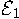
\includegraphics[]{E1.pdf}
	&
	$\begin{aligned}[t] % placement: default is "center", options are "top" and "bottom"
	\vect{\kappa b}_{2i-1} 	& =  \frac{2}{L_{i-1}} \vect{u}_{2i-2} \times \vect{u}_{2i-1}\\[0.5em]
	\vect{\kappa b}_{2i+1} 	& =  \frac{2}{L_{i}} \vect{u}_{2i} \times \vect{u}_{2i+1}
	\end{aligned}$
\end{tabularx}


\subsubsection{Unit tangent vector at ghost vertices}
% ---------------------------------------------------------------------

This definition of the curvature leads to a natural definition of the unit tangent vector at ghost vertex $\vect{x}_{2i-1}$ (resp. $\vect{x}_{2i+1}$), as the unit vector tangent to the osculating circle of the ($i-1$)th segment (resp. $i$th segment) at that point.

\begin{tabularx}{\textwidth}[t]{>{\centering\arraybackslash}m{0.48\textwidth} >{\centering\arraybackslash}X} % >{\centering\arraybackslash}
	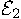
\includegraphics[]{E2.pdf}
	&
	$\begin{aligned}[t] % placement: default is "center", options are "top" and "bottom"
	\vect{t}_{2i-1}	&=  \frac{l_{2i-1}}{L_{i-1}} \vect{u}_{2i-2}	+ 	\frac{l_{2i-2}}{L_{i-1}} \vect{u}_{2i-1} 	\\[0.5em]
	\vect{t}_{2i+1} 	&=  \frac{l_{2i+1}}{L_{i}} \vect{u}_{2i}		+ 	\frac{l_{2i}}{L_{i}} \vect{u}_{2i+1}
	\end{aligned}$
\end{tabularx}

\subsubsection{Left/right unit tangent vector at handle vertices}
% -----------------------------------------------------------------------------------
Equivalently, the definition of the osculating circles of the ($i-1$)th and $i$th segments leads to a natural definition of the left ($\vect{t}_{2i}^-$) and right ($\vect{t}_{2i}^+$) unit tangent vectors at handle vertex $\vect{x}_{2i}$, for segments of uniform curvature. When both segments have the same curvature, left and right vectors agree.

\begin{tabularx}{\textwidth}[t]{>{\centering\arraybackslash}m{0.48\textwidth} >{\centering\arraybackslash}X} % >{\centering\arraybackslash}
	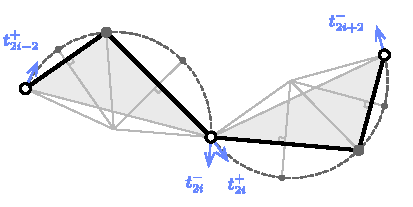
\includegraphics[]{E3.pdf}
	&
	$\begin{aligned}[t] % placement: default is "center", options are "top" and "bottom"
	\vect{t}_{2i}^- 	&= 2 (\vect{t}_{2i-1} \cdot \vect{u}_{2i-1}) \vect{u}_{2i-1} - \vect{t}_{2i-1} \\[0.5em]
	\vect{t}_{2i}^+ 	&= 2 (\vect{t}_{2i+1} \cdot \vect{u}_{2i}) \vect{u}_{2i} - \vect{t}_{2i+1}
	\end{aligned}$
\end{tabularx}

\subsubsection{Unit tangent vector at handle vertices}
% ----------------------------------------------------------------------
The unit tangent vector $\vect{t}_{2i}$ (that is the cross-section normal) at handle vertex $\vect{x}_{2i}$ is chosen to be the mean of the left and right unit tangent vectors at that vertex.\footnote{Consequently, this model assumes that the field of tangents along the centerline is continuous and is thus unable to model cases where the centerline is not at least $\mathcal{C}^1$. In such case the beam must be considered as two parts glued together.}

\begin{tabularx}{\textwidth}[t]{>{\centering\arraybackslash}m{0.48\textwidth} >{\centering\arraybackslash}X} % >{\centering\arraybackslash}
	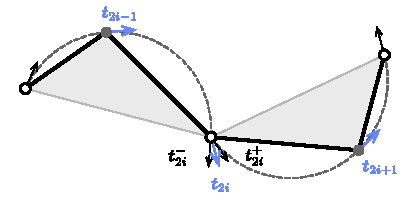
\includegraphics[]{E4.pdf}
	&
	$\begin{aligned}[t] % placement: default is "center", options are "top" and "bottom"
	\vect{t}_{2i} 	&= \frac{\vect{t}_{2i}^- + \vect{t}_{2i}^+ }{\norm{\vect{t}_{2i}^- + \vect{t}_{2i}^+}}
	\end{aligned}$
\end{tabularx}

This way, the determination of the tangent vectors (or equivalently the section normals) in the static equilibrium configuration will be done in the flow of the Dynamic Relaxation process, without the need of introducing any additional degrees of freedom (for instance the usual Euler angles). The position of the vertices rules the orientation of the cross-section normals.

\subsubsection{Left/right bending moment at handle vertices}
% ---------------------------------------------------------------------------------
Given the unit tangent vector $\vect{t}_{2i}$, one can define the left ($\vect{\kappa}_{2i}^-$) and right ($\vect{\kappa}_{2i}^+$) curvature at handle vertex $\vect{x}_{2i}$. The left curvature is initially evaluated from the left osculating circle, defined as the circle passing through $\vect{x}_{2i-1}$ and $\vect{x}_{2i}$ and tangent to $\vect{t}_{2i}$ at $\vect{x}_{2i}$. The right curvature is initially evaluated from the right osculating circle, defined as the circle passing through $\vect{x}_{2i}$ and $\vect{x}_{2i+1}$ and tangent to $\vect{t}_{2i}$ at $\vect{x}_{2i}$.\footnote{Remark that the centerline is now approximated with a biarc in the vicinity of $\vect{x}_{2i}$. This is the reason why this model is called the \textquote{biarc model}.}${}^,$\footnote{This model offers the ability to represent discontinuities in curvature -- thus in bending moment -- at handle vertices as the left and right curvatures does not necessarily agree. This is quite different from the classical 3-dof element~\cite{Barnes1999, Adriaenssens1999, Douthe2006} which assumes that the curvature -- thus the bending moment -- is $\mathcal{C}^0$ and can be evaluated at every vertices from the circumscribed osculating circle.}

\begin{tabularx}{\textwidth}[t]{>{\centering\arraybackslash}m{0.48\textwidth} >{\centering\arraybackslash}X} % >{\centering\arraybackslash}
	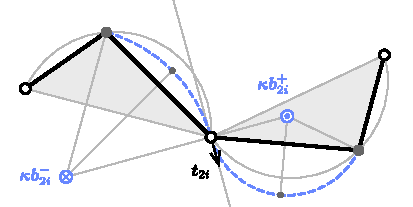
\includegraphics[]{E5.pdf}
	&
	$\begin{aligned}[t] % placement: default is "center", options are "top" and "bottom"
	\vect{\kappa b}_{2i}^- &=  \frac{2}{l_{2i-1}} \vect{u}_{2i-1} \times \vect{t}_{2i}
	\\[0.5em]
	\vect{\kappa b}_{2i}^+ &=  \frac{2}{l_{2i}} \vect{t}_{2i} \times \vect{u}_{2i}
	\end{aligned}$
\end{tabularx}

However, this values need to be adjusted so that the static condition for rotational equilibrium is satisfied at all time ($\vect{M}^{ext}  + \vect{M}^+ - \vect{M}^- = 0$). Therefore, this condition will be satisfied in particular at the end of the solving process. To achieve this goal, we first compute a realistic mean value ($\vect{M}_{2i}^{\perp}$) for the internal bending moment as~:
\begin{equation}
		\vect{M}_{2i}^{\perp}	=  \frac{1}{2} \mat{B}_{i-1}(\vect{\kappa b}_{2i}^- - \rconf{\vect{\kappa b}}_{2i}^-)
					+  \frac{1}{2} \mat{B}_{i}(\vect{\kappa b}_{2i}^+ - \rconf{\vect{\kappa b}}_{2i}^+)
\end{equation}
To enforce the jump discontinuity in bending moment ($\vect{M}^{ext} = \vect{M}^- - \vect{M}^+$) across the handle vertex, we define the left and right bending moments at $\vect{x}_{2i}$ as~:
\begin{subequations}
	\begin{align}
		{\vect{M}_{2i}^{\perp}}^{-} &=  \vect{M}_{2i}^{\perp}	 + \frac{1}{2} \vect{M}_{2i}^{\perp,\;ext}
		\\[0.5em]
		{\vect{M}_{2i}^{\perp}}^{+} &=   \vect{M}_{2i}^{\perp}	 - \frac{1}{2} \vect{M}_{2i}^{\perp,\;ext}
	\end{align}
	\label{eq:DeltaM}
\end{subequations}
Note that in the case where no external concentrated bending moment is applied to the handle vertex, the internal bending moment is continuous across the vertex as expected.

\subsubsection{Left/right curvature at handle vertices}
% --------------------------------------------------------------------
Finally, the left and right curvature at handle vertex $\vect{x}_{2i}$ are computed back with the constitutive law~:
\begin{subequations}
	\begin{align}
		\vect{\kappa b}_{2i}^-  &=  \mat{B}_{i-1}^{\;-1} {\vect{M}_{2i}^{\perp}}^{-} + \rconf{\vect{\kappa b}}_{2i}^-
		\\[0.5em]
		\vect{\kappa b}_{2i}^+  &=  \mat{B}_{i}^{\;-1} {\vect{M}_{2i}^{\perp}}^{+} + \rconf{\vect{\kappa b}}_{2i}^+
	\end{align}
\label{eq:lr_bending_moment}
\end{subequations}

\subsubsection{Bending moment at ghost vertices}
% -----------------------------------------------------------------
The internal bending moment at ghost vertices is simply given by the constitutive law as~:
\begin{subequations}
	\begin{align}
		\vect{M}_{2i-1}^{\perp} &=  \mat{B}_{i-1}(\vect{\kappa b}_{2i-1} - \rconf{\vect{\kappa b}}_{2i-1})
		\\[0.5em]
		\vect{M}_{2i+1}^{\perp} &=  \mat{B}_{i}(\vect{\kappa b}_{2i+1} - \rconf{\vect{\kappa b}}_{2i+1})
	\end{align}
\end{subequations}

\subsection{Discret rate of twist and twisting moment}
% =======================================
We assume the twisting moment and the rate of twist to vary linearly over $]\vect{x}_{2i},  \vect{x}_{2i+2}[$.
Thus, the material twist of the rod at mid edge is given by~:
\begin{subequations}
	\begin{align}
		\tau_{i+1/2} = \frac{\Delta\theta_{i}}{{l}_i}\label{eq:d_twist}
		\\[0.5em]
		\varkappa_{3,\,i+1/2} = \frac{\Delta\theta_{i}}{\rconf{l}_i}\label{eq:d_twist}
	\end{align}
\end{subequations}
To compute $\Delta\theta_{i} = \theta_{i+1} - \theta_{i}$ imagine that the rod is framed with a Bishop frame $\{\vect{u},\vect{v},\vect{t}\}$. Because the material frame $\{\vect{d}_1,\vect{d}_2,\vect{d}_3\}$ is also adapted to the rod centerline, it can be transformed into the Bishop frame with a single rotation of angle $\theta(s)$ around $\vect{d}_3(s) =\vect{t}(s)$. Because the Bishop frame does not twist around $\vect{d}_3$, the rate of change of angle $\theta$ along the curve directly leads to the computation of the rate of twist as exposed in \cref{eq:d_twist}.

In the discrete case, although it is possible to frame the whole curve with a Bishop frame to achieve the computation of the rate of twist \cite{Lefevre2017}, it is more convenient to measure $\Delta\theta_{i}$ step by step using the existing material frames at vertices $\vect{x}_i$ and $\vect{x}_{i+1}$. This is done in a two step process :
\begin{enumerate}
\item
Parallel transport the material frame $\{\vect{d}_{1,i},\vect{d}_{2,i},\vect{d}_{3,i}\}$ at vertex $\vect{x}_i$ onto vertex $\vect{x}_{i+1}$. We call $\{\vect{d}_{1,i}^{\para}, \vect{d}_{2,i}^{\para},\vect{d}_{3,i}^{\para}\}$ the resulting frame positioned at $\vect{x}_{i+1}$ such that $\vect{d}_{3,i}^{\para} = \vect{d}_{3,i+1}$.
\item
Measure $\Delta\theta_{i} = \angle{(\vect{d}_{1,i}^{\para},\vect{d}_{1,i+1})} = \angle{(\vect{d}_{2,i}^{\para},\vect{d}_{2,i+1})}$ as the oriented angle needed to align $\vect{d}_{1,i}^{\para}$ with $\vect{d}_{1,i+1}$ (or $\vect{d}_{2,i}^{\para}$ with $\vect{d}_{2,i+1}$) by a rotation of angle $\Delta\theta_{i}$ around $\vect{d}_{3,i+1} = \vect{t}_{i+1}$.
\end{enumerate}
Consequently, the twisting moment at mid span of each edge is computed directly with the appropriate constitutive equation :
\begin{subequations}
	\begin{alignat}{3}
	\vect{Q}_{2i+1/2} &= Q_{2i+1/2}\, \vect{u}_{2i} \quad &&\text{where} \quad {Q_{2i+1/2}} = GJ_i(\varkappa_{3,\,2i+1/2} - \rconf{\varkappa}_{3,\,2i+1/2})
	\\
	\vect{Q}_{2i+3/2} &= Q_{2i+3/2}\, \vect{u}_{2i+1}\quad &&\text{where} \quad {Q_{2i+3/2}} = GJ_i(\varkappa_{3,\,2i+3/2} - \rconf{\varkappa}_{3,\,2i+3/2})
	\end{alignat}
\end{subequations}
Remark the sign convention~: as expected, when edge $\vect{e}_i$ suffers a positive twist ($\varkappa_{3,\,i+1/2} > 0$), frame $\{\vect{d}_{1,i+1},\vect{d}_{2,i+1},\vect{d}_{3,i+1}\}$ makes frame $\{\vect{d}_{1,i},\vect{d}_{2,i},\vect{d}_{3,i}\}$ to rotate positively around $\vect{u}_i$ as $Q_{i+1/2} > 0$.

% Discret shear force
% --------------------------
\subsection{Discret shear force}
Recall that in Kirchhoff's theory the shear force is a reacting parameter, computed from the equilibrium equations and not from a constitutive law. Firstly, remark that the shear force can be factorized under the following expression~:
\begin{equation}
	\vect{F}^{\perp} = F_1 \vect{d}_1 + F_2 \vect{d_2} = - \vect{d}_3 \times (\vect{d}_3 \times \vect{F}) \label{eq:shearid}
\end{equation}
Then, combining \cref{eq:motion_4,eq:motion_5} --~where the inertial terms are neglected~-- with \cref{eq:shearid} leads to the following vectoriel form of the shear force~:
\begin{equation}
	\vect{F}^{\perp}
	= (1+\epsilon)^{-1} \vect{d}_3 \times \left(\frac{\partial \vect{M}}{\partial s} + \vect{m} \right)
	=  \vect{d}_3 \times \left(\frac{\partial \vect{M}}{\partial s_t} + \frac{\vect{m}}{1+\epsilon} \right)
	\label{eq:shear}
\end{equation}
In the discrete case, the shear force is evaluated at mid span of each edge by :
\begin{subequations}
	\label{eq:dshear}
	\begin{alignat}{3}
		&\vect{F}^{\perp}_{2i+1/2}
		=  \vect{u}_{2i} &&\times \left( \frac{\vect{M}_{2i+1} - \vect{M}_{2i}^{+}}{l_{2i}}+ \frac{\rconf{l}_{2i}}{l_{2i}} \vect{m}_i \right)
		\label{eq:dshear_a}
		\\[0.5em]
		&\vect{F}^{\perp}_{2i+3/2}
		=  \vect{u}_{2i+1} &&\times \left( \frac{\vect{M}_{2i+2}^- - \vect{M}_{2i+1}}{l_{2i+1}}+ \frac{\rconf{l}_{2i+1}}{l_{2i+1}} \vect{m}_i \right)
		\label{eq:dshear_b}
	\end{alignat}
\end{subequations}
Remark that the derivative of the internal moment at mid edge is evaluated by the finite difference of the moment between the two closest vertices. This is in accordance with the quadratic interpolation method of a vector-valued function given in \cref{ch:interpolation}.

Expressed in the form of \cref{eq:dshear_a,eq:dshear_b}, the discrete shear force has the interesting property to remain strictly orthogonal to $\vect{d}_{3,i+1/2} = \vect{u}_i$. While this is true in the continuous world, this property can easily be lost in the discrete case where mean values and derivatives are evaluated through finite summations or finite differences.

%Equivalent equations could be expressed in a scalar form derived from \cref{eq:dshear_a,eq:dshear_b} as~:
%\begin{subequations}
%	\begin{alignat}{3}
%		&F_{1,\;2i+1/2}  =  \frac{\rconf{l}_{2i}}{l_{2i}}
%		 \left(
%		 -\frac{M_{2,\,2i+1} - M_{2,\,2i}^{+}}{\rconf{l}_{2i}}
%		 - \varkappa_{3,\,2i+1/2}M_{1,\,2i+1/2}
%		 +\varkappa_{1,\,2i+1/2}Q_{2i+1/2}
%		 \right)
%		\\[0.5em]
%		&\vect{F}^{\perp}_{2i+3/2}
%		=  \vect{u}_{2i+1} &&\times \left( \frac{\vect{M}_{2i+2}^- - \vect{M}_{2i+1}}{l_{2i+1}}+ \frac{\rconf{l}_{2i+1}}{l_{2i+1}} \vect{m}_i \right)
%		\label{eq:dshear_b}
%	\end{alignat}
%\end{subequations}

\subsubsection{Matrix notation}
Because there is a derivation with respect to $s$ in \cref{eq:dshear_a,eq:dshear_b}, one must be very careful when writing these equations in matrix notation. Indeed, their counterparts will translate differently wether the symbols will be decomposed in the \emph{global} frame basis or in the \emph{material} frame basis.

If the symbols are decomposed in the \emph{global} frame basis the translation is straightforward as the derivative of a vector is the vector of the derived components~:
\begin{equation}
	\vect{M} = {\begin{bmatrix}M_x \\ M_y \\ M_z\end{bmatrix}}
	\quad , \quad
	\vect{M}'
	=
	{\begin{bmatrix}M_x \\ M_y \\ M_z\end{bmatrix}}^{'}
	=
	\begin{bmatrix}M_x' \\ M_y' \\ M_z'\end{bmatrix}
\end{equation}
Thus, in the discrete case, the evaluation of the derivative of the moment at mid-edge is achieved thanks to the finite difference formula~:
\begin{equation}
	\vect{M}'_{2i+1/2}
	\simeq
	\frac{1}{\rconf{l}_{2i}}\left( {\begin{bmatrix}M_x & M_y & M_z\end{bmatrix}}_{2i+1}^T - {\begin{bmatrix}M_x & M_y & M_z\end{bmatrix}}_{2i}^T \right)
\end{equation}
However, if the symbols are given in the \emph{material} frame basis, the derivation must take into account the spatial velocity $\vect{\varkappa}$ of the material frame~:
\begin{equation}
	\vect{M} = {\begin{bmatrix}M_1 \\ M_2 \\ Q \end{bmatrix}}
	\quad , \quad
	\vect{M}'
	=
	{\begin{bmatrix}
	M_1 \\ M_2 \\ Q
	\end{bmatrix}}^{'}
	=
	\begin{bmatrix}
	M_1' \\ M_2' \\ Q'
	\end{bmatrix}
	+
	\begin{bmatrix}
	\varkappa_1 \\ {\varkappa_2} \\ \varkappa_3
	\end{bmatrix}
	\times
	\begin{bmatrix}
	M_1 \\ M_2 \\ Q
	\end{bmatrix}
\end{equation}
Thus, in the discrete case, the evaluation of the derivative of the moment at mid-edge is still achieved thanks to the finite difference formula, but takes a very different matrix form~:
\begin{equation}
	\begin{aligned}
	\vect{M}'_{2i+1/2}
	&\simeq
	&&\frac{1}{\rconf{l}_{2i}}\left( {\begin{bmatrix}M_1 & M_2 & Q\end{bmatrix}}_{2i+1}^T - {\begin{bmatrix}M_1 & M_2 & Q\end{bmatrix}}_{2i}^T \right)
	\\
	&+ &&\frac{1}{2}\left( {\begin{bmatrix}\varkappa_1 & \varkappa_2 & \varkappa_3\end{bmatrix}}_{2i}^T + {\begin{bmatrix}\varkappa_1 & \varkappa_2 & \varkappa_3\end{bmatrix}}_{2i+1}^T \right)
	\\
	&\times
	&& \frac{1}{2} \left( {\begin{bmatrix}M_1 & M_2 & Q\end{bmatrix}}_{2i}^T + {\begin{bmatrix}M_1 & M_2 & Q\end{bmatrix}}_{2i+1}^T \right)
	\end{aligned}
\end{equation}
Although this paragraph could seem superfluous to the reader, this point is a matter of concern when implementing the model into an algorithm. Indeed, the developper always has the choice between two natural data structures where vectors are represented by a triplet either in the global frame basis or in the material frame basis (see \cref{eq:stiffnessmatrix}). Even more, he can decide to mix the two for practical reasons, for instance if it leads to less arithmetic computations. In particular, the stiffness matrix has a nice diagonal shape when written in the material frame basis. Thus it seems desirable to do the computation of the bending moment in this basis. On the contrary, we have just seen that it seems easier to compute the shear force in the global frame basis.

\subsection{Interpolation of the internal forces and moments}
At this point, for a given geometric configuration, we know how to compute the bending moment at vertices. But we only know how to compute the twisting moment, the axial force and the shear force at mid edges. However, our final goal is to describe the discrete rod as a particle-spring system were mass is lumped at vertices and elements are modeled as interactions between vertices. In this representation, all actions must be resumed to vertex actions, the only conceptual entity that will have a meaning to the dynamic process.

Therefore, we need to express the value of the twisting moment, the axial force and the shear force at vertices and not only at mid edges. This can be done using \cref{eq:motion} were the inertial member is set to zero, that is neglecting the inertial forces. Although this is not exactly true during the dynamic of the rod, it is exactly true at static equilibrium, the only state we are interested in.

\subsubsection{Axial force}
From \cref{eq:motion_3} we evaluate the variation of the axial force over a segment $]\vect{x}_{i},  \vect{x}_{i+1}[$ and deduce the variation of the axial strain from the constant axial stiffness $ES_i$ of the segment~:
\begin{subequations}
	\begin{alignat}{2}
		&\Delta N_{i+1/2} &&= -l_i  \cdot {[\varkappa_1 F_2 - \varkappa_2 F_1 + f_3]}_{i+1/2}
		\label{eq:DeltaN}
		\\
		&\Delta \epsilon_{i+1/2} &&= \Delta N_{i+1/2} / {ES}_i
	\end{alignat}
\end{subequations}
Then we conclude on the expression of the axial force at vertices~:
\begin{subequations}
	\begin{alignat}{2}
		&N_{i}^{+} &&= N_{i+1/2} - \frac{1}{2} \Delta N_{i+1/2}  \\[0.5em]
		&N_{i+1}^{-} &&= N_{i+1/2} + \frac{1}{2} \Delta N_{i+1/2}
	\end{alignat}
	\label{eq:dNi}
\end{subequations}
and the expression of the axial strain at vertices~:
\begin{subequations}
	\begin{alignat}{2}
		&\epsilon_{i}^{+} &&= \epsilon_{i+1/2} - \frac{1}{2} \Delta \epsilon_{i+1/2}  \\[0.5em]
		&\epsilon_{i+1}^{-} &&= \epsilon_{i+1/2} + \frac{1}{2} \Delta \epsilon_{i+1/2}
	\end{alignat}
\end{subequations}
Remark how a distributed external axial force (${f}_3$) modifies the value of the axial component of the internal force at vertices, and thus is taken into account in the final static equilibrium.

\subsubsection{Shear force}
From \cref{eq:motion_1,eq:motion_2} we evaluate the variation of the shear force over a segment $]\vect{x}_{i},  \vect{x}_{i+1}[$ ~:
\begin{subequations}
	\begin{alignat}{2}
		&\Delta F_{1,\,i+1/2}^{} &&= - l_i  \cdot {[\varkappa_2 F_3 - \varkappa_3 F_2 + f_1]}_{i+1/2}
		\\
		&\Delta F_{2,\,i+1/2}^{} &&= - l_i  \cdot {[\varkappa_3 F_1 - \varkappa_1 F_3 + f_2]}_{i+1/2}
	\end{alignat}
	\label{eq:DeltaF}
\end{subequations}
Then we conclude on the expression of the shear force components at vertices~:
\begin{subequations}
	\label{eq:dFi}
	\begin{alignat}{2}
		&F_{1,\,i}^{+} &&= F_{1,\,i+1/2} - \frac{1}{2} \Delta F_{1,\,i+1/2}  \\[0.5em]
		&F_{1,\,i+1}^{-} &&= F_{1,\,i+1/2} + \frac{1}{2} \Delta F_{1,\,i+1/2} \\[0.5em]
		&F_{2,\,i}^{+} &&= F_{2,\,i+1/2} - \frac{1}{2} \Delta F_{2,\,i+1/2}  \\[0.5em]
		&F_{2,\,i+1}^{-} &&= F_{2,\,i+1/2} + \frac{1}{2} \Delta F_{2,\,i+1/2}
	\end{alignat}
\end{subequations}
Remark how a distributed external shear force ($\vect{f}^{\perp} = f_1\vect{d}_1 + f_2\vect{d}_2$) modifies the value of the shear components of the internal force at vertices, and thus is taken into account in the final static equilibrium.

\subsubsection{Twisting moment}
From \cref{eq:motion_6} we evaluate the variation of the twisting moment over a segment $]\vect{x}_{i},  \vect{x}_{i+1}[$ and deduce the variation of twist from the constant torsional stiffness $GJ_i$ of the segment~:
\begin{subequations}
	\begin{alignat}{2}
		&\Delta Q_{i+1/2} &&= -l_i  \cdot {[\varkappa_1 M_2 - \varkappa_2 M_1 + m_3]}_{i+1/2}
		\label{eq:DeltaQ}
		\\
		&\Delta \varkappa_{3,\,i+1/2} &&= \Delta Q_{i+1/2} / {GJ}_i
	\end{alignat}
\end{subequations}
Then we conclude on the expression of the twisting moment at vertices~:
\begin{subequations}
	\begin{alignat}{2}
		&Q_{i}^{+} &&= Q_{i+1/2} - \frac{1}{2} \Delta Q_{i+1/2}  \\[0.5em]
		&Q_{i+1}^{-} &&= Q_{i+1/2} + \frac{1}{2} \Delta Q_{i+1/2}
	\end{alignat}
	\label{eq:dQi}
\end{subequations}
and the expression of the rate of twist at vertices~:
\begin{subequations}
	\begin{alignat}{2}
		&\varkappa_{3,\,i}^{+} &&= \varkappa_{3,\,i+1/2} - \frac{1}{2} \Delta \varkappa_{3,\,i+1/2}  \\[0.5em]
		&\varkappa_{3,\,i+1}^{-} &&= \varkappa_{3,\,i+1/2} + \frac{1}{2} \Delta \varkappa_{3,\,i+1/2}
	\end{alignat}
\end{subequations}
Remark how a distributed external twisting moment ($m_3$) modifies the value of the axial component of the internal moment at vertices, and thus is taken into account in the final static equilibrium.

\section{Dynamic Relaxation}\label{sec=DR}
From the previous section we have established the basis for a discrete rod element that can account for extension, flexion and torsion. This element is made of two types of vertices~: the ghost and the handle vertices. This allows to model discontinuities at handle vertices, which is one of the main contribution of the work exposed in this chapter. We have established a precise \dofs{4} discrete geometric representation of a slender rod. And from a given configuration we have learned to compute the internal forces and moments acting on the rod vertices using Kirchhoff's theory. Therefore, we are able to compute the resultant of the internal force and moment acting on a given vertex of the rod.\footnote{Note that the internal forces and moments embed the action of distributed external forces and moments applied to the rod.}

We now expose a process to find the static equilibrium of a rod, which is our ultimate goal. This process is called \emph{Dynamic Relaxation} and was first introduced by \citef{Day1965}. We assume that we know the stress-free configuration of the rod, its material and cross-section properties. The rod might also be subjected to known external loads such as climatic loads. Finally, we call initial configuration the actual configuration of the rod at time $t=0$. In this configuration, the rod is (a priori) not at static equilibrium.

\subsection{Overview of the procedure}
In the Dynamic Relaxation procedure, a discretized mechanical system is dropped from a known initial configuration at time $t=0$. Technically speaking, the mechanical system is now idealized to a \emph{particle-spring system} where each vertex is assimilated to a \emph{particle}, also called \emph{node}, represented by a material frame. Each particle has its own mass and is subjected to internal and external forces and moments. Because the system is not yet in a state of static equilibrium, the internal forces does not equilibrate the external forces. Thus, the system is subject to a motion. This motion is integrated through time and artificially damped. When all the kinetic energy is dissipated by the damping the system has reached a state of static equilibrium, which is the steady state response of the system.

Because the motion is only a mean to find a static equilibrium position of the system, the damping does not need to be realistic and should be chosen so that the system approaches the static position as fast as possible. This is also known as \emph{critical damping}.

\subsection{Resultants acting on a particle}\label{sec=resFM}
In this section, we express the resultant force and the resultant twisting moment acting on a particle. If not balanced, these resultants will make the particle to move and rotate with respect to its degrees of freedom $\vect{x}$ and $\theta$.

\subsubsection{Resultant force}
The translational resultant force ($\vect{R}_i^x$) acting on a particle is the sum of two contributions. The first one ($\vect{F}_i^{ext}$) is the resultant of the concentrated forces applied to the particle such as climatic loads, support reactions or loads transferred through connections. The second one ($\vect{F}_i^{int}$) is the resultant of the internal forces applied by the upstream and downstream parts of the rod to the particle and are given by \cref{eq:dNi,eq:dFi}. This leads to the following equations~: \footnote{Recall the convention from \cref{fig:rodslice}~: the internal force and moment are chosen to be the action of the downstream part of the rod upon the upstream part of the rod.}
\begin{subequations}
\begin{alignat}{2}
	&\vect{R}_i^x &&= \vect{F}_i^{int} + \vect{F}_i^{ext}
	\\
	&\vect{F}_i^{int} &&= - \vect{F}_i^{-} + \vect{F}_i^{+}
	\\
	& \vect{F}_i^{-}  &&= F_{1,\,i}^{-} \,\vect{d}_{1,\,i}  + F_{2,\,i}^{-} \,\vect{d}_{2,\,i} + N_i^- \,\vect{d}_{3,\,i}
	\\
	&\vect{F}_i^{+}  &&= F_{1,\,i}^{+} \,\vect{d}_{1,\,i}  + F_{2,\,i}^{+} \,\vect{d}_{2,\,i} + N_i^+ \,\vect{d}_{3,\,i}
\end{alignat}
\end{subequations}
Note that the contribution of the distributed external forces ($\vect{f}_i^{}$) is already taken into account via the interpolation of the internal force (see \cref{eq:DeltaN,eq:DeltaF}). Likewise, the contribution of the distributed external bending moment ($\vect{m}_i^{\perp}$) is also taken into account via the calculation of the internal shear force (see \cref{eq:dshear}). Finally, the contribution of the concentrated external bending moments is yet included via the expression of the discrete shear force (see \cref{eq:DeltaM,eq:dshear}).

\subsubsection{Resultant twisting moment}
In the same manner, the resultant twisting moment ($R_i^{\theta}$) acting on a particle is the sum of two contributions.\footnote{Actually, $R_i^{\theta}$ is the component of the resultant moment along $\vect{d}_{3,\,i}$. We only need to compute this component as we have only one rotational degree of freedom in our model.} The first one ($Q_i^{ext}$) is the resultant of the concentrated twisting moments applied to the particle. The second one (${Q}_i^{int}$) is the resultant of the internal twisting moment applied by the upstream and downstream parts of the rod to the particle and given by \cref{eq:dQi}. This leads to the following equations~:
\begin{subequations}
\begin{alignat}{2}
	&{R}_i^{\theta} &&= {Q}_i^{int} + {Q}_i^{ext}
	\\
	&{Q}_i^{int} &&= - {Q}_i^{-} + {Q}_i^{+}
\end{alignat}
\end{subequations}
Note that the contribution of the distributed external twisting moment ($q_i^{ext}$) is already taken into account via the interpolation of the internal twisting moment (see \cref{eq:DeltaQ}).

\subsection{Equations of motion}
The particles of the system evolve according to the laws of motion, with respect to the 4 degrees of freedom of the system ($\vect{x}$ and $\theta$), given by~:
\begin{subequations}
\label{eq:dmotion}
\begin{alignat}{3}
	& m_i^x\; \ddot{\vect{x}}_i  + \lambda^x_i \dot{\vect{x}}_i && = \vect{R}_i^x \label{eq:dmotion_a}
	\\
	& m_i^{\theta} \; \ddot{\theta}_i + \lambda^{\theta}_i \dot{\theta}_i&& = R_i^{\theta} \label{eq:dmotion_b}
\end{alignat}
\end{subequations}
where $\ddot{\vect{x}}_i$ is the translational acceleration of the particle, $\ddot{\theta}_i$ is the rotational acceleration of the particle and $\lambda^x_i$ and  $\lambda^{\theta}_i$ are the viscous damping coefficients.

Hereinafter we will consider no viscous damping. Instead, we will rely on an artificial kinetic damping (see \cref{sec=damping}). For a detailed traitement of various damping methods in the Dynamic Relaxation method refer to \cite{Underwood1983,Rezaiee2012}.

\subsubsection{Coupling between flexion and torsion}
Although \cref{eq:dmotion_a,eq:dmotion_b} may seem uncoupled to the reader, it is not the case as the coupling occurs through the material frame (see \cref{sec=dofchain}). Recall that both $\vect{R}_i^x$ and $R_i^{\theta}$ do depend on the $\vect{x}_i$ and $\theta_i$ variables.

\subsubsection{Nonlinearity}
In a linear analysis the expression of the resultant force and the resultant moment would be linearized and written in the matrix form~:
\begin{subequations}
\begin{alignat}{3}
	& \mat{M}^x\; \mat{\ddot{X}}  + \mat{\lambda}^x \mat{\dot{X}} && = \mat{K}^x \mat{X}
	\\
	& \mat{M}^{\theta} \; \mat{\ddot{\Theta}} + \mat{\lambda}^{\theta} \mat{\dot{\Theta}}&& =  \mat{K}^{\theta}\mat{\Theta}
\end{alignat}
\end{subequations}
where $\mat{X}$ and $\mat{\Theta}$ are the column vectors of the translational ($\vect{x}_i$) and rotational ($\theta_i$) degrees of freedom of the system~; $\mat{M}^{x}$ and $\mat{M}^{\theta}$ are the mass matrices~; $\mat{\lambda}^{x}$ and $\mat{\lambda}^{\theta}$ are the damping matrices and $\mat{K}^x$ and $\mat{K}^{\theta}$ are the stiffness matrices.\footnote{For non linear simulation, the stiffness matrix is replaced by the \emph{tangent} stiffness matrix and is reevaluated at each time step.}

Saying that the system is linearized involves that the dependence of $\vect{R}_i^x$ and $R_i^{\theta}$ with respect to the degrees of freedom $\vect{x}_i$ and $\theta_i$ will be modeled as a (linear) matrix product and that $\mat{K}^x$ and $\mat{K}^{\theta}$ are computed independently of these variables. In other words, this means that $\vect{R}_i^x$ and $R_i^{\theta}$ are calculated as a linear combination of the degrees of freedom, and that the coefficients of this combination are the matrix entries of
$\mat{K}^x$ and $\mat{K}^{\theta}$.

Here, this factorization is not possible. $\vect{R}_i^x$ and $R_i^{\theta}$ are computed from the degrees of freedom of the system but the relation is not linear (see how the internal force and moment are computed in \cref{sec=dmodel}). Therefore, the geometric system given in \cref{eq:dmotion_a,eq:dmotion_b} is effectively nonlinear.

\subsection{Explicit time integration}

In this section, we give the stages required to integrate these equations through time. The Dynamic Relaxation procedure is based on a central-difference scheme. We call $\dt{}$ the time step. And we call \emph{initial configuration} the configuration of the system at time $t=0$.

Note that the time step $\dt{}$ is not necessary constant through time and could be \emph{adapted} during the analysis process. However, for simplicity we will treat only the case where it is constant but it is easy to extend the present work to work with a variable time step.

\subsubsection{Acceleration}
At time $t$, considering the position of the system is known ($\vect{x}_i$ and $\{\vect{d}_{3,\,i},\vect{d}_{1,\,i},\vect{d}_{2,\,i}\}$), we can compute the resultant force ($\vect{R}_i^x$) and the resultant twisting moment ($R_i^{\theta}$) acting on the particles (see \cref{sec=resFM}). Using \cref{eq:dmotion} the acceleration of the particles at time $t$ is straightforwardly deduced as~:
\begin{subequations}
\label{eq:da}
\begin{alignat}{3}
	& \ddot{\vect{x}}_i^t && = \frac{\vect{R}_i^{x,\,t}}{m_i^x}
	\\[0.5em]
	& \ddot{\theta}_i^t && = \frac{R_i^{\theta,\,t}}{m_i^{\theta}}
\end{alignat}
\end{subequations}

\subsubsection{Velocity}
The translational and rotational velocities of a particle are evaluated with the following central difference scheme~:
\begin{subequations}
\begin{alignat}{3}
	& \ddot{\vect{x}}_i^t && =\frac{\dot{\vect{x}}_i^{t+\dt{} / 2} - \dot{\vect{x}}_i^{t-\dt{} / 2}}{\dt{}}
	\\[0.5em]
	& \ddot{\theta}_i^t && = \frac{\dot{\theta}_i^{t+\dt{} / 2} - \dot{\theta}_i^{t-\dt{} / 2}}{\dt{}}
\end{alignat}
\end{subequations}
where $\dot{\vect{x}}_i$ and $\dot{\theta}_i$ are the translational and rotational velocities of the particle. Thus, the velocity of a particle at time $t + \dt{} / 2$ is computed from its velocity at time $t - \dt{} / 2$ by~:
\begin{subequations}
\label{eq:dv}
\begin{alignat}{5}
	& \dot{\vect{x}}_i^{t+\dt{} / 2} &&
	=  \dot{\vect{x}}_i^{t-\dt{} / 2}
	&&+ \dt{}  \cdot \frac{\vect{R}_i^{x,\,t}}{m_i^x}
	\\[0.5em]
	& \dot{\theta}_i^{t+\dt{} / 2} &&
	=  \dot{\theta}_i^{t-\dt{} / 2}
	&&+ \dt{}  \cdot \frac{R_i^{\theta,\,t}}{m_i^{\theta}}
\end{alignat}
\end{subequations}

\subsubsection{Position}
To update the position of the system, we use the same central difference scheme but this time on the velocity~:
\begin{subequations}
\begin{alignat}{3}
	& \dot{\vect{x}}_i^{t+h/2} && =\frac{{\vect{x}}_i^{t} - {\vect{x}}_i^{t-\dt{}}}{\dt{}}
	\\[0.5em]
	& \dot{\theta}_i^{t+h/2} && = \frac{{\theta}_i^{t} - {\theta}_i^{t-\dt{}}}{\dt{}}
\end{alignat}
\end{subequations}
Thus, the translational and rotational positions of a particle at time $t + \dt{}$ are computed from the velocities at time $t + \dt{} / 2$ by~:
\begin{subequations}
\label{eq:dx}
\begin{alignat}{5}
	& \vect{x}_i^{t+\dt{}}
	&& =  \vect{x}_i^{t} + \dt{}  \cdot  \dot{\vect{x}}_i^{t+\dt{} / 2}
	\\[0.5em]
	& {\theta}_i^{t+\dt{}}
	&& =  {\theta}_i^{t} + \dt{}  \cdot  \dot{{\theta}}_i^{t+\dt{} / 2}
\end{alignat}
\end{subequations}
Using \cref{eq:dv} the position at time $t+\dt{}$ can be expressed with respect to the position, velocity and resultants computed at time $t$ as~:
\begin{subequations}
\label{eq:dx2}
\begin{alignat}{5}
	& \vect{x}_i^{t+\dt{}}
	&& =  \vect{x}_i^{t} + \dt{} \cdot \dot{\vect{x}}_i^{t-\dt{} / 2}
	&&+ {\dt{}}^2  \cdot \frac{\vect{R}_i^{x,\,t}}{m_i^{x}}
	\\[0.5em]
	& {\theta}_i^{t+\dt{}}
	&& =  {\theta}_i^{t} + \dt{}  \cdot  \dot{{\theta}}_i^{t- \dt{} / 2}
	&&+ {\dt{}}^2  \cdot \frac{R_i^{\theta,\,t}}{m_i^{\theta}}
\end{alignat}
\end{subequations}

\subsubsection{Motion}
From this new position, it is now possible to compute the new resultant force and moment acting on the particles, to update their acceleration, then to update their velocity, and then to compute the new position of the system, at time $t + 2\dt{}$. This process can be repeated indefinitely to follow the motion of the system.

\subsubsection{Initialization}
The iterative process described in this section to simulate step by step the motion of the system needs to be initialized. At the moment, \cref{eq:dx2} only describes how to get the position of the system at $t + \dt{}$ knowing its position, velocity and acceleration at time $t$.

At time $t=0$, or each time that the system will be damped (see \cref{sec=damping}), we consider that the system is released with no initial velocity, which means that~:
\begin{subequations}
\begin{alignat}{3}
	& \dot{\vect{x}}_i^{0} && = \frac{\vect{x}_i^{-\dt{}/2} + \vect{x}_i^{+\dt{}/2}}{2}
	\quad \Rightarrow \quad
	 \dot{\vect{x}}_i^{-\dt{} / 2}   = -  \dot{\vect{x}}_i^{+\dt{} / 2}
	\\[0.5em]
	& \dot{\theta}_i^{0} && = \frac{\theta_i^{-\dt{}/2} + \theta_i^{+\dt{}/2}}{2}
	\quad \Rightarrow \quad
	\dot{\theta}_i^{-\dt{} / 2}   = - \dot{\theta}_i^{+\dt{} / 2}
\end{alignat}
\end{subequations}
Therefore, the velocity at time $\dt{} / 2$ given in \cref{eq:dv} becomes~:
\begin{subequations}
\label{eq:dv0}
\begin{alignat}{5}
	& \dot{\vect{x}}_i^{+\dt{} / 2} &&
	=  \frac{1}{2} \dt{}  \cdot \frac{\vect{R}_i^{x,\,t}}{m_i^x}
	\\[0.5em]
	& \dot{\theta}_i^{+\dt{} / 2} &&
	=  \frac{1}{2} \dt{}  \cdot \frac{R_i^{\theta,\,t}}{m_i^{\theta}}
\end{alignat}
\end{subequations}
and the next position at time $t + \dt{}$ is still computed from \cref{eq:dx}.
\subsubsection{Error propagation}
Note that the motion will be realistic to the extent that the computed forces and moments will be realistic and to the extent that the time step will be small enough. Indeed, at each time step an approximation error is done in the evaluation of the velocity and the position of the system with the central difference scheme. This error is integrated through time and nothing here is done to correct it and to prevent its accumulation during the dynamic. It is not a matter of concern for us as we are only interested in the quasi-static response of the system and not in an accurate modeling of the system's motion. Moreover, higher accuracy numerical integrators would be more computationally expensive, which is against our goal to achieve real-time interactive simulation of elastic gridshells.

Lots of other integration schemes exist, among which we can cite the \emph{Explicit Euler}, the \emph{Symplectic Euler}, the \emph{Störmer-Verlet} and the \emph{4\textsuperscript{th} order Runge-Kutta} schemes. These schemes are briefly presented in \cite{Fierz2013}. For a complete treatment of numerical integrators refer to the book from \citef{Hairer2006}.

\subsection{Damping}\label{sec=damping}
If no damping is introduced to dissipate some energy, there is no reason that the system will stop to move. Here, our goal is to dissipate the kinetic energy of the system as fast as possible to fall into a state of static equilibrium. This can be achieved with any kind of damping, among which the most well-known are \emph{viscous damping} and \emph{kinetic damping}.

Here, we choose to implement the kinetic damping as it is known to produce the best results for a wide range of cases \cite{Rezaiee2012}.

\subsubsection{Kinetic damping}
Kinetic damping was first introduced by \citef{Cundall1976}. The idea behind this type of damping is simple. For a conservative system, the mechanical energy ($\mathcal{E}_m$) is conserved during motion and is the sum of two forms of energy~: the potential energy ($\mathcal{E}_p$) and the kinetic energy ($\mathcal{E}_k$). Therefore, the potential energy of the system is minimized when its kinetic energy is maximized.

To find a state of static equilibrium, that is a state of minimal potential energy, Cundall proposes to track the kinetic energy of the system during motion. When a peak is detected, the system is frozen in its position and then released with no initial velocity, that is with no initial kinetic energy. When the system is released, the overall mechanical energy of the system has decreased and is all stocked under potential energy form. The motion starts again and part of the initial potential energy is converted to kinetic energy, until a new peak is detected. Progressively, from peak to peak, the potential energy is progressively lowered to a minimum and the system falls in a state of static equilibrium.

Because of the discrete nature of the numerical process, a peak of kinetic energy is detected in the interval $[t-3\dt{}/2,\,t+\dt{}/2]$ when (see \cref{fig:ek_interp})~:
\begin{equation}
	\mathcal{E}_k^{t-\dt{}/2} >  \mathcal{E}_k^{t+\dt{}/2}
\end{equation}
where the kinetic energy of the system is computed from the mass and the velocity of the particles by~:
\begin{subequations}
\label{eq:Ek}
\begin{alignat}{5}
	& \mathcal{E}_k^{x,\,t-\dt{}/2} && =  \sum_i \tfrac{1}{2} m_i^x \dot{\vect{x}}_i^{t-\dt{} / 2}
	\\[0.5em]
	& \mathcal{E}_k^{\theta,\,t-\dt{}/2} && = \sum_i \tfrac{1}{2} m_i^{\theta} \dot{{\theta}}_i^{t-\dt{} / 2}
	\\[0.5em]
	& \mathcal{E}_k^{t-\dt{}/2} && = \mathcal{E}_k^{x,\,t-\dt{}/2} + \mathcal{E}_k^{\theta,\,t-\dt{}/2}
\end{alignat}
\end{subequations}
Here, we have made the distinction between the translational part of the kinetic energy ($\mathcal{E}_k^{x}$) and the rotational part of the kinetic energy ($\mathcal{E}_k^{\theta}$). Indeed, the kinetic damping can be triggered either considering the global kinetic energy of the system or considering separately the translational and rotational parts of the kinetic energy of the system.\footnote{That is when a peak of $\mathcal{E}_k^{x}$ or a peak of $\mathcal{E}_k^{\theta}$ is detected the kinetic damping is triggered.}


\subsubsection{Peak interpolation}
When a peak is detected at time $t+\dt{} /2$, the simplest way to proceed is to froze the system in its actual position, at time $t$, and to release it from this position with no initial velocity. However, the peak of kinetic energy as occurred at time $t^*$ somewhere in between times $t-\dt{}/2$ and $t+\dt{}/2$. To maximise the effect of the kinetic damping the position of the peak could be guessed using a parabolic interpolation of the kinetic energy.

\begin{figure}[t]
%\begin{fullpage}
     	\centering
     	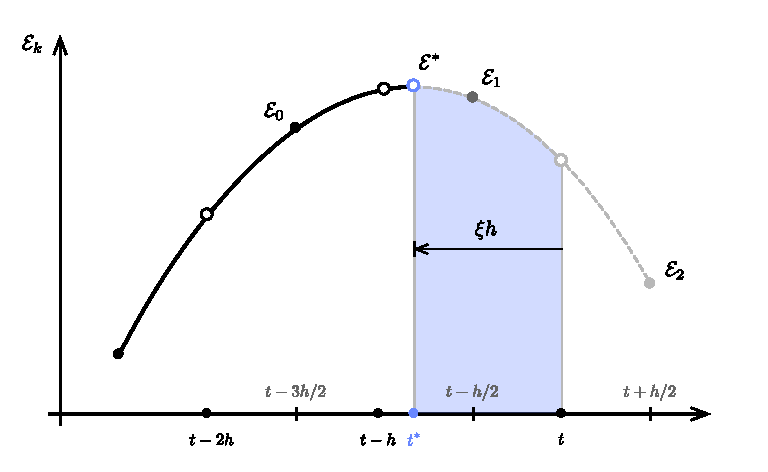
\includegraphics{Ek_interpolation.pdf}
	\captionof{figure}[Parabolic interpolation of the kinetic energy peak]{Parabolic interpolation of the kinetic energy peak.}
	\label{fig:ek_interp}
%\end{fullpage}
\end{figure}

Let us define $\mathcal{E}_0$, $\mathcal{E}_1$ and $ \mathcal{E}_2$ the last three consecutive values of the kinetic energy~:
\begin{subequations}
\begin{alignat}{5}
	& \mathcal{E}_0 &&= \mathcal{E}_k^{t-3\dt{}/2}
	\\[0.5em]
	& \mathcal{E}_1 &&= \mathcal{E}_k^{t-\dt{}/2}
	\\[0.5em]
	& \mathcal{E}_2 &&= \mathcal{E}_k^{t+\dt{}/2}
\end{alignat}
\end{subequations}
Because a peak has just occurred, the following inequalities hold~:
\begin{subequations}
\begin{alignat}{5}
	& \mathcal{E}_1 \geqslant \mathcal{E}_0
	\\
	& \mathcal{E}_1 \geqslant \mathcal{E}_2
\end{alignat}
\end{subequations}
We define the following parameters for the parabolic interpolation of the kinetic energy~:
\begin{subequations}
\label{eq:InterpParam}
\begin{alignat}{5}
	& \alpha = \frac{\mathcal{E}_1 - \mathcal{E}_0}{\mathcal{E}_1 - \mathcal{E}_2} \geqslant 0
	\\[0.5em]
	& \xi = \frac{\mathcal{E}_2 - \mathcal{E}_1}{\mathcal{E}_0 - 2\mathcal{E}_1 + \mathcal{E}_2} = \frac{1}{1 + \alpha} \in [0,1]
\end{alignat}
\end{subequations}
With these parameters, the position of the peak and the value of the kinetic energy at the peak are given by~:
\begin{subequations}
\label{eq:InterpEk}
\begin{alignat}{5}
	& t^* &&= t - \xi t
	\\[0.5em]
	& \mathcal{E}^* &&= \mathcal{E}_1 + \frac{1-2\xi}{8} (\mathcal{E}_2 - \mathcal{E}_0)  \geqslant \mathcal{E}_1
\end{alignat}
\end{subequations}
Observe that $1-2\xi$ and $\mathcal{E}_2 - \mathcal{E}_0$ have the same sign. Therefore, $\mathcal{E}^*$ is always greater than $\mathcal{E}_1$ as expected. The system is then pushed backward to the interpolated position $\vect{x}_i^*$ and $\theta_i^*$ given by~:
\begin{subequations}
\label{eq:InterpX}
\begin{alignat}{5}
	& \vect{x}_i^{*}
	&& =  \vect{x}_i^{t} && -\xi \dt{}  \cdot  \dot{\vect{x}}_i^{t-\dt{} / 2}
	\\[0.5em]
	& {\theta}_i^{*}
	&& =  {\theta}_i^{t} && -\xi \dt{}  \cdot  \dot{{\theta}}_i^{t-\dt{} / 2}
\end{alignat}
\end{subequations}
These equations can be advantageously rewritten to minimize memory allocation by avoiding the storage of the position and the speed of the system respectively at time $t-\dt{}$ and $t-\dt{} / 2$~:
\begin{subequations}
\label{eq:InterpX2}
\begin{alignat}{5}
	& \vect{x}_i^{*}
	&& =  \vect{x}_i^{t} -\xi   \dt{}  \cdot (\dot{\vect{x}}_i^{t+\dt{} / 2} - {\dt{}} \cdot \frac{\vect{R}_i^{x,\,t}}{m_i^x} )
	\\[0.5em]
	& {\theta}_i^{*}
	&& =  {\theta}_i^{t} -\xi \dt{} \cdot (\dot{{\theta}}_i^{t+\dt{} / 2} - {\dt{}}  \cdot \frac{R_i^{\theta,\,t}}{m_i^{\theta}})
\end{alignat}
\end{subequations}
The parabolic interpolation was introduced by \citef{Barnes1999}. The advantage of this technique is double. Firstly, the damping occurs at the interpolated position, that is for a higher level of kinetic energy ($\mathcal{E}^* \geqslant \mathcal{E}_1$, see \cref{fig:ek_interp}). Hence, more kinetic energy is dissipated which should improve the convergence speed. Secondly, because of the interpolation, the system is less subject to \emph{time step locking} when the system moves back and forth between two positions.

\subsection{Convergence}
Several criteria exist in the literature to determine when to stop the time integration and to decide wether the algorithm has converged to a state of static equilibrium or not. It is very unlikely that the system will fall exactly in such a state. Instead it will only get close to it an so a \emph{convergence criteria} is required. We recall here the main ideas.

\subsubsection{Criterion based on the resultant force}
The system is at static equilibrium when all nodes are at static equilibrium. Thus, it is possible to test for convergence looking at the nodal residuals $\norm{\vect{R}_i^{x,\,t}}$ and $\norm{\vect{R}_i^{\theta,\,t}}$.\footnote{Here, the $\norm{}$ symbol denotes the usual Euclidian norm for vectors.} For instance, convergence could be pronounced when the maximum of the residuals is less than a certain amount of force ($R_{\epsilon}^x$) and moment ($R_{\epsilon}^{\theta}$)~:
\begin{subequations}
\begin{alignat}{5}
	& \max_{i}{\norm{\vect{R}_i^{x,\,t}}}  \leqslant R_{\epsilon}^x
	\\[0.5em]
	& \max_{i}{\norm{{R}_i^{\theta,\,t}}}  \leqslant R_{\epsilon}^{\theta}
\end{alignat}
\end{subequations}
It can be found that this criterion is too strict and it might be preferable to rely on a more global criterion, for instance by testing the mean residual~:
\begin{subequations}
\label{eq:meancrit}
\begin{alignat}{5}
	& \frac{1}{N} \sum_{i}{\norm{\vect{R}_i^{x,\,t}}}  \leqslant R_{\epsilon}^x
	\\[0.5em]
	& \frac{1}{N} \sum_{i}{\norm{{R}_i^{\theta,\,t}}}  \leqslant R_{\epsilon}^{\theta}
\end{alignat}
\end{subequations}
where $N$ is the number of particles in the system. This approach is easily extended to any norm or generalized mean acting on the vector of residuals. For instance the $p$\,-mean could be an appropriate criterion~:
\begin{subequations}
\label{eq:meancrit_g}
\begin{alignat}{5}
	& \left(\frac{1}{N} \sum_{i}{\norm{\vect{R}_i^{x,\,t}}^p} \right)^{1/p}
	\leqslant R_{\epsilon}^x
	\\[0.5em]
	& \left(\frac{1}{N}  \sum_{i}{\norm{{R}_i^{\theta,\,t}}^p}  \right)^{1/p}
	\leqslant R_{\epsilon}^{\theta}
\end{alignat}
\end{subequations}
Recall that when $p=-1$ it is called the \emph{harmonic mean}, when $p=1$ it is called the \emph{arithmetic mean} and when $p=2$ it is called the \emph{quadratic mean}.

\subsubsection{Criterion based on the velocity}
The system is at static equilibrium when it does not move anymore, that is when the velocity of the system remains null. Thus, it is possible to test for convergence looking at the nodal velocities $\norm{\vect{\dot{x}}_i^t}$ and $\norm{\dot{\theta}_i^t}$. The same kind of criteria can be formed.

\subsubsection{Criterion based on the displacement}
Displacement criteria are very similar to velocity criteria. The convergence is pronounced when the displacement of the system is considered negligible. The same kind of criteria can be formed.

\subsubsection{Criterion based on the kinetic energy}
The kinetic energy can also be employed to form convergence criteria. Somehow, it is nothing but a velocity criteria weighted by the fictitious mass of the particles. It makes sens as particles contribute to the motion proportionally to their mass. All the criteria exposed previously can be formed with the kinetic energy $\tfrac{1}{2} m_i^x \dot{\vect{x}}_i^{t}$ and $\tfrac{1}{2} m_i^{\theta} \dot{{\theta}}_i^{t}$ of the particles.

\subsubsection{Relative and adaptative criterion}
It can be useful to proportionate the convergence criteria to the size of the system. For the same level of convergence a system with 1000 elements is likely to have a higher kinetic energy than a system with 1 element. The first answer to this issue is to consider a mean value over the particles, as proposed in \cref{eq:meancrit,eq:meancrit_g}.

Some authors have proposed another option to address this problem \cite{Barnes1975,Douthe2007}. They define the kinetic energy convergence threshold as a fraction ($f$) of the maximum kinetic energy observed previously during the motion~:
\begin{subequations}
\begin{alignat}{5}
	& \sum_i \tfrac{1}{2} m_i^x \dot{\vect{x}}_i^{t}
	&& \leqslant f \cdot \max_{[0,t]} \mathcal{E}_{k}^{x,\,t}
	\\[0.5em]
	& \sum_i \tfrac{1}{2} m_i^{\theta} \dot{{\theta}}_i^{t}
	&& \leqslant f \cdot  \max_{[0,t]} \mathcal{E}_{k}^{\theta,\,t}
\end{alignat}
\end{subequations}
Hence, this criterion is \emph{adaptative} and also \emph{relative} to the size of the problem. The same approach can be adopted for force, velocity or displacement based criteria.

%Expliquer l'interpolation des efforts. Il y a un choix a faire dans la DR. Soit on écrit l'équilibre sur le noeud (de dimension null). Soir on écrit l'équilibre sur une tranche de dimension $l_i+l{i+1}/2$. Mais si l'on veut maintenir la précision des conditions de passage, la DR fonctionne avec des noeuds et pas des tranches, le mieux est d'opter pour un équilibre du noeud. La DR va minimiser les résidus aux noeuds et donc on aura les bonnes conditions de passage sous Fext et Mext. J'ai montré que la convergence était plus rapide et précise. On a pas de décalage dans les diagrammes des efforts (si il y en a, ce sont uniquement les défauts de convergence, le résidu , n'étant pas strictement nul au noeud à la fin de la DR).

\subsection{Stability and critical damping}\label{sec=stab_crit}
Because we are not interested by the motion itself but by the quasi-static response of the system when properly damped, the time step ($\dt{}$) and the mass of the particles ($m_i^x$, $m_i^{\theta}$) should be chosen in order~:
\begin{itemize}
\item to ensure that the algorithm will converge to a state of static equilibrium (stability)~;
\item to produce the fastest convergence possible (critical damping).
\end{itemize}

\subsubsection{Translational fictitious mass}

\citef{Barnes1999} studies the vibration modes of a simple unidimensional mass-spring system to postulate that the optimal fictitious mass of a particle is related to the time step and the stiffness lumped at the particle by~:
\begin{equation}
	m_i = \frac{h^2}{2} K_i
\end{equation}
A demonstration of this result is proposed by \citef{Papadrakakis1981} and \citef{Underwood1983} for an automatic evaluation of the fictitious mass of the particles. $K_i$ should be understood as the greatest direct stiffness that can occur during the simulation process at the $i$th particle. For a structure with only tension and compression members, Barnes computes the stiffness lumped at a particle according to the geometric and material stiffness of all the members ($j$) that are connected to this particle~:
\begin{equation}
	K_i = \sum_j \Bigl[\frac{ES}{L_0} + g \frac{N}{L} \Bigr]
\end{equation}
$ES/L_0$ is the axial stiffness of the element while $N/L$ is its geometric stiffness. Because the geometric stiffness varies along the simulation, Barnes introduces a multiplication factor ($g > 1$). This factor must be chosen by the end user to ensure that when $gN/L$ is evaluated it is effectively an upper bound to $N/L$ at all time.

\citef{Douthe2007} extends the formulation of Barnes to account for flexural stiffness~:
\begin{equation}
	\frac{h^2}{2} \sum_j \Bigl[\frac{ES}{L_0} + g \left(\frac{N}{L} + \frac{EI}{L^3} \right) \Bigr]
\end{equation}
In practice, the bending stiffness is negligible in front of the axial stiffness. Additional informations can be found in \cite{Lewis2003,Rodriguez2011a}.

\subsubsection{Rotational fictitious mass}
By analogy to these works and following \cite{Lefevre2017} we define the twisting fictitious mass as~:
\begin{equation}
	K_i = \sum_j \Bigl[\frac{GJ}{L_0} + g \frac{Q}{L} \Bigr]
\end{equation}

\subsubsection{Fictitious mass update}
In practice, as remarked in \cite{Douthe2007} the fictitious masses do not evolve a lot between two peaks of kinetic energy. Therefore, they can be reevaluated only after each peak to minimize the computational cost of the algorithm.

\subsection{Application to the simple plane pendulum}
The simple pendulum -- where a weight is suspended from a pivot so that it can swing freely -- is of practical interest to illustrate how the Dynamic Relaxation procedure works. We recall the analytical solution for this nonlinear problem. We then explore the progress of the Dynamic Relaxation method to find the position of static equilibrium of the pendulum.

\subsubsection{Equation of motion}
Let us call $m$ the mass and $l$ the length of the pendulum (see \cref{fig:pendulum}). The angle $\theta(t)$ gives the position of the pendulum at time $t$ from the vertical axis. The motion of the pendulum is given by the following differential equation~:
\begin{equation}
	\ddot{\theta} + {\omega_0}^2 \sin{\theta} = 0 \label{eq:nlpendulum}
\end{equation}
In addition, we call $\theta_0 = \theta(0)$ the initial position of the pendulum where it is dropped with no initial velocity ($\dot{\theta}(0) = 0$). Remark that $m$ is not involved in \cref{eq:nlpendulum}.\footnote{We could have introduced a fictitious mass ($m_f$) for the weight to optimize the convergence of the algorithm (see \cref{sec=stab_crit}). In this case, the reference pulsation of the pendulum would writes~: $\omega_0 = \sqrt{(m/m_f)\cdot(g/l)}$. The real mass of the weight is the one that give access to the force exerted to the pendulum while the fictitious mass is freely chosen to speed up the convergence of the method.}

The kinetic, potential and mechanical energies of the pendulum are given by~:
\begin{subequations}
\begin{alignat}{5}
	&\mathcal{E}_k = \frac{1}{2} m \dot{\theta}^2
	\\
	&\mathcal{E}_p =  mgl (1-\cos\theta)
\end{alignat}
\end{subequations}
\subsubsection{Linearization for small oscillations}
For a small initial angle ($\theta_0 \ll 1$) \cref{eq:nlpendulum} simplifies to~:
\begin{equation}
	\ddot{\theta} + {\omega_0}^2 {\theta} = 0 \label{eq:lpendulum}
\end{equation}
and the period $T_0$ and the angular frequency $\omega_0$ of the pendulum are given by~:
\begin{subequations}
\begin{alignat}{5}
	&{T_0} &&= \frac{2\pi}{\omega_0}\\[0.5em]
	&{\omega_0} &&= \left({\frac{g}{l}}\right)^{1/2}
\end{alignat}
\end{subequations}
Therefore, for small angles the period is independent of the initial angle $\theta_0$.

\subsubsection{Exact solution}
For greater initial angles, the solution is nonlinear and requires elliptic functions to be solved analytically \cite{Borghi2013,Belendez2007}.

The period of the pendulum is given in terms of the elliptic integral $K$ by~:
\begin{subequations}
\begin{alignat}{5}
	&T / T_0  = \frac{2}{\pi}K(k)
	\\[0.5em]
	& k = \sin (\theta_0 / 2)
	\\[0.5em]
	&K(m) = \int_0^1 \frac{dz}{\sqrt{(1-z^2)(1-mz^2)}}
\end{alignat}
\end{subequations}
The position of the pendulum over time is expressed in terms of the \emph{Jacobi elliptic function} $sn(u,m)$ by~:
\begin{equation}
	\theta(t) = 2 \arcsin \Bigl( k \,sn(\omega_0\cdot(T/4 - t), k) \Bigr)
\end{equation}
The angular velocity of the pendulum is calculated from the conservation of mechanical energy as~:
\begin{equation}
	\dot{\theta}(t) = 2 \omega_0 \Bigl( \sin^2 (\theta_0/2) - \sin^2 (\theta/2) \Bigr)^{1/2}
\end{equation}

\begin{figure}[p]
	\centering
\begin{fullpage}
   \subfloat[][First steps until the first peak of $\mathcal{E}_k$ is reached]{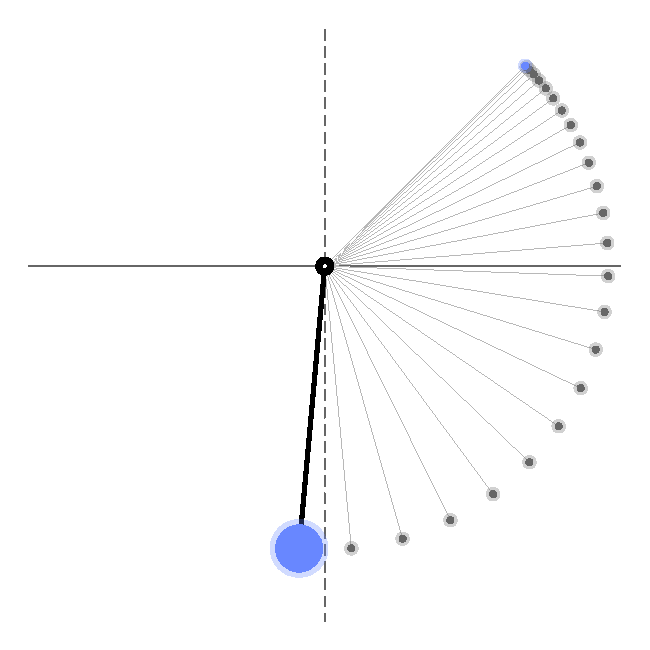
\includegraphics[width=100mm]{pendulum.pdf}\label{fig:pendulum}} \\
   \subfloat[][Potential energy of the pendulum for the first steps]{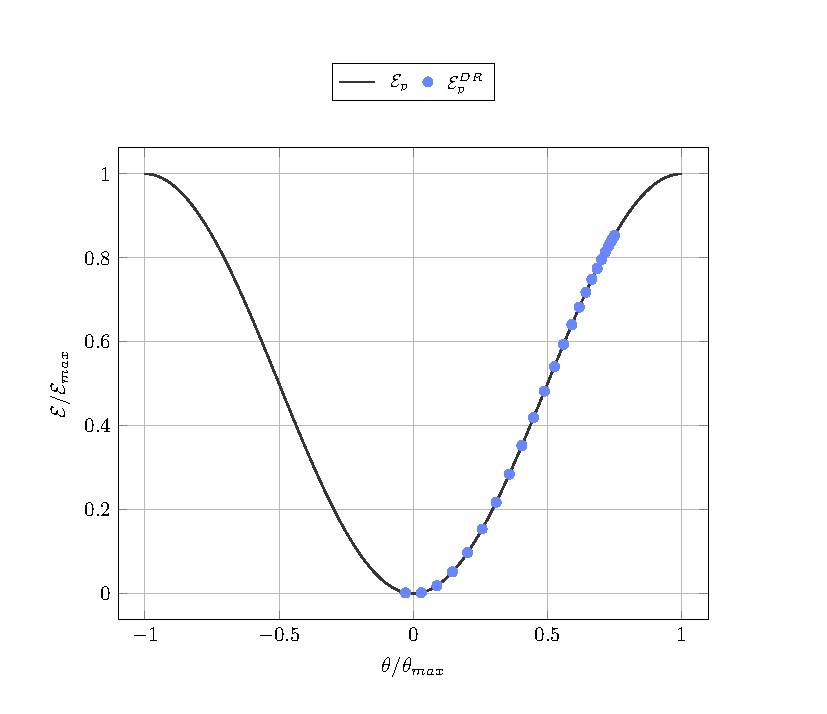
\includegraphics[width=120mm]{ch7_numeric/plot/1_pendulum/build_Ep.pdf}\label{fig:pendulum_Ep}}
   \vspace{10pt}
   \captionof{figure}[]{Application of the DR process to the simple plane pendulum.}
\end{fullpage}
\end{figure}
\begin{figure}[p]
	\centering
\begin{fullpage}
   \subfloat[][Typical profile of the kinetic damping]{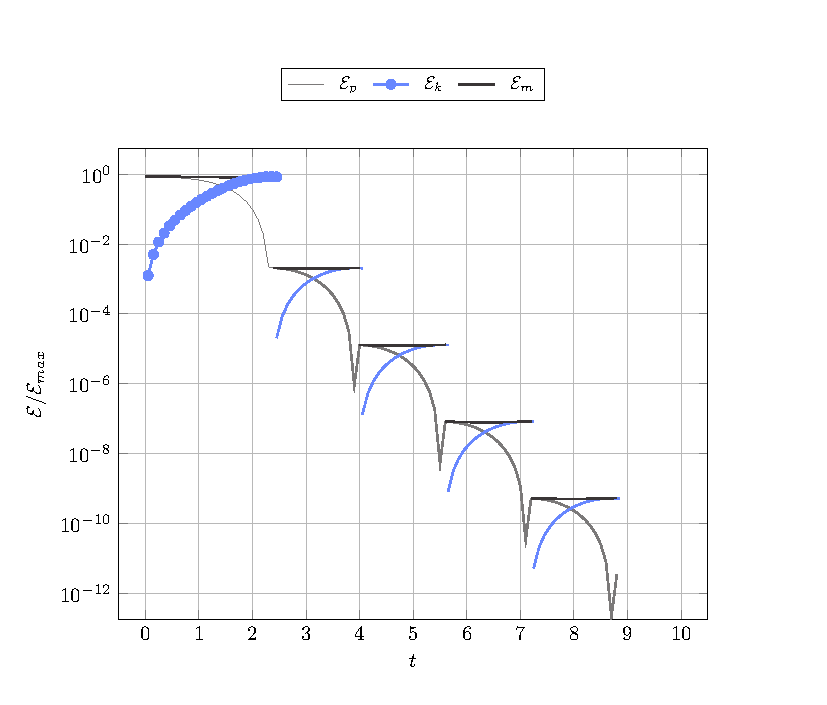
\includegraphics[width=120mm]{ch7_numeric/plot/1_pendulum/build_Ek.pdf}\label{fig:pendulum_Ek}} \\
   \subfloat[][Convergence of the DR process in the phase space]{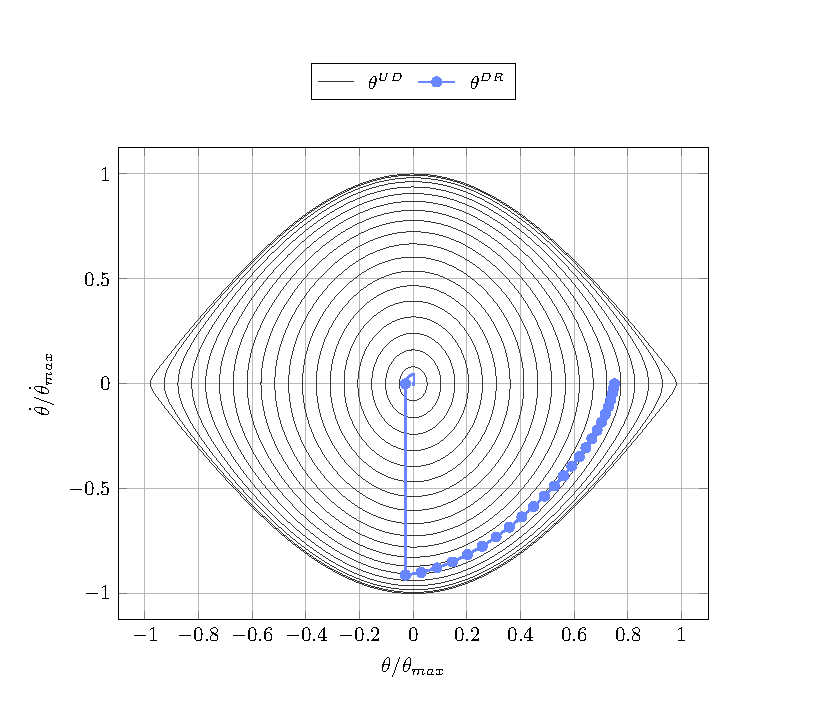
\includegraphics[width=120mm]{ch7_numeric/plot/1_pendulum/build_Phase.pdf}\label{fig:pendulum_Phase}} \\
   \vspace{10pt}
   \captionof{figure}[]{Convergence of the DR process for the simple plane pendulum.}
\end{fullpage}
\end{figure}

\subsubsection{Finding the position of static equilibrium}
A pendulum of mass $m = \SI{1.0}{kg}$ is dropped with no initial velocity at angle $\theta_0 = \SI{135}{\degree}$. The length of the pendulum is defined so that its angular frequency is $\omega_0 = \SI{1.0}{s^{-1}}$. The gravity is $g = \SI{9.81}{m/s^2}$.

The motion of the pendulum is simulated by the Dynamic Relaxation method with kinetic damping. Interpolation of kinetic energy peaks is not implemented in this example. When a peak is detected, the pendulum is pushed backward to its previous position, frozen and dropped again with no initial velocity. The time step is set to $h = \SI{0.1}{s}$ and the simulation is stopped when the kinetic energy of the pendulum is less than $\mathcal{E}_k^{lim} = 10^{-20}$.

The course of the pendulum for the first iterations is represented in \cref{fig:pendulum}. The pendulum is dropped with no velocity at angle $\theta_0$. Driven by the gravity, it starts to move down slowly and its velocity increases over time. Progressively, its potential energy is transformed into kinetic energy but the overall mechanical energy is conserved because the motion is undamped until a peak of kinetic energy is reached (see \cref{fig:pendulum_Ek}).

The potential energy of the pendulum decreases until it reaches the vertical axis (see \cref{fig:pendulum_Ep}). But because of the discrete nature of the algorithm, the pendulum jumps over the equilibrium position and starts to move up few time steps. Accordingly its velocity starts to decrease and so its kinetic energy. Quickly, a peak of kinetic energy is deteced and the kinetic damping is triggered.

The process is repetead but with a lower initial position $\theta_0$. The mechanical energy of the system has decreased and so has the upper bound of the potential energy. From peak to peak, this bound is lowered through kinetic damping and in the end the potential energy of the pendulum is reduced to zero within the convergence tolerance $\mathcal{E}_k^{lim}$ (see \cref{fig:pendulum_Ek}).

The convergence process is also monitored with the phase diagram of the motion (see \cref{fig:pendulum_Phase}). Each closed curve is an iso-curve which corresponds to a given level of mechanical energy defined by $\mathcal{E}_m = \mathcal{E}_p(\theta_0)$. An undamped pendulum travels along an iso-curve and makes a full turn every period of time $T$. Here, until a kinetic energy peak is reached the level of mechanical energy is preserved during the motion and the pendulum moves along the corresponding iso-curve in the phase diagram.

Observe in \cref{fig:pendulum_Phase} that the pendulum slightly deviates from its theoretical movement. The velocity is slightly under estimated from its theoretical value. This error is due to the central difference approximation of the velocity and is integrated during the motion, thus accumulating over time. When the kinetic damping is triggered this error is dissipated. This kind of diagram is very useful to compare time integrators as proposed in \cite{Hairer2006}. In the phase diagram, the effect of the kinetic damping is to jump from one iso-curve to another with a lower mechanical energy level (see \cref{fig:pendulum_Phase}).

This application is also useful to understand the relation between accuracy, stability and critical damping~:
\begin{itemize}
\item When $h \ll T$ the method sticks closely to the theoretical movement. The process is stable and peaks of kinetic energy are determined with accuracy. However the method requires a huge amount of iterations which increases the computation time.
\item When $h \gg T$ the method gets unstable as the dynamic is updated at a lower rate than the typical reaction time of the system. The process fails to capture a plausible motion and bolting is likely to occur. In this case the pendulum will start to swirl.
\end{itemize}


\section{Enriching the model}\label{sec=enriching}

The question of support conditions and connexions are often kept quiet when a beam model is presented. But it is of critical concerned when modeling real structures which always have to be fixed somewhere or connected to other structural components. Usually these conditions have a preponderant influence on the overall mechanical behavior of a structure and therefore must not be neglected.

One of the main motivations of our work was precisely to develop an element that is capable of modeling real complex bending-active structures, and which can take account of a rich variety of support conditions and connections. The preliminary work done on the geometry of curves -- spent to build a comprehensive understanding of how tangent vectors and curvature can be interpreted at vertices and especially at end vertices (see \cref{chp=curve}) -- was essential to achieve our goal.

\subsection{Support condition}
There exists two major ways of modeling support conditions, compatible with the dynamic relaxation procedure~:
\begin{itemize}
\item Enforce the condition by means of velocity constraints.
\item Enforce the condition by means of return forces and moments.
\end{itemize}

In terms of implementation, when you need to block a specific degree of freedom, either reset its velocity to zero in the dynamic process or apply an additional external force to nullify the resultant of forces and moments applied to that node so it won't move. While both options are valid, it seems that the last one as the advantage to require the explicit computation of the \emph{support reaction} -- that is the return force or moment applied by the support to the particle so it does not move (with respect to a certain degree of freedom).

Also notice that we can identify three types of boundary conditions~:
\begin{itemize}
\item \emph{Rigid}, when a support prevents the particle from moving along a given degree of freedom.
\item \emph{Elastic}, when a support applies a return force or moment proportional to the displacement of the particle.
\item \emph{Free}, when no support exists and the particle is free to move.
\end{itemize}
Remarque that a \emph{Free} boundary condition is by extension an \emph{Elastic} boundary condition with an infinitely low stiffness.

In the dynamic relaxation procedure, the tangent vectors are computed from the position of the particles except at the endings where an indecision remains. At these vertices, either ~:
\begin{itemize}
\item The position of the tangent vector is fixed because the cross-section is clamped (i.e. \emph{rigid} boundary condition) and the bending moment is deduced from \cref{eq:cir_kb_ends}.
\item The end bending moment is prescribed (i.e. \emph{free} or \emph{elastic}) and the tangent vector is obtained by inverting \cref{eq:lr_bending_moment,eq:cir_kb_ends}.
\end{itemize}
If the bending moment is prescribed -- either $\vect{M}^{\perp} = 0$ for a \emph{free} end or $\vect{M}^{\perp}\neq 0$ for an elastic support -- the corresponding tangent is deduced from \cref{eq:lr_bending_moment,eq:cir_kb_ends} by :
\begin{subequations}
\setlength{\jot}{8pt}
\begin{alignat}{2}
	&\vect{\kappa b}_{0} &&= \mat{B}_{0}^{-1} \vect{M}_{0}^{\perp} +  \rconf{\vect{\kappa b}}_{0} \\
	&\vect{t}_0 &&= \left(1 - \left(\frac{l_0 \kappa_0}{2}\right)^2\right)\vect{u}_0
		-  \frac{l_0 \kappa_0}{2} \;\vect{\kappa b}_{0} \times \vect{u}_0
\end{alignat}
\end{subequations}
Note that as expected $\vect{t}_0$ is perpendicular to $\vect{\kappa b}_{0}$. A similar relation can be deduced for $\vect{t}_n$.

\subsection{Connection}
A connection between several beams can usually be interpreted as a set of geometric constraints involving two or more particles. There exists two major ways of modeling connections, compatible with the dynamic relaxation procedure~:
\begin{itemize}
\item The first approach is to enforce the constraint \emph{smoothly} through a set of mechanical actions, namely forces and moments. In that case, the connection is equivalent to a sort of spring, not necessarily linear, and there is conceptually no difference with what an element really is (see for instance \cite{Lefevre2017}).
\item The second approach is to enforce the constraint \emph{brutally} through a reprojection process. That is after each time step the configuration of the system is perturbed so it conforms to the constraints prescribed by the definition of the connexions (see for instance \cite{Douthe2007,DAmico2014}).
\end{itemize}

The last option is straightforward to implement for constraints on translational \dofs{} but more complex to resolve for constraints on rotational \dofs{}. The advantage is that the solution is always valid regarding these constraints. On the contrary, brutal projection can leads to numerical \emph{hysteresis locking} when the system switch back and forth between two configurations, one after and one before the reprojection procedure.

The first option seems more natural to implement and more meaningfull mechanically speaking. The distance between the actual and target configurations of the connection is evaluated and leads to (proportional) return forces and moments acting on the \dofs{6} particles involved in the constraint. Because the connection acts similarly to an element, it must be taken into account in the computation of the fictitious mass of the particles. Moreover, the stiffness of the connection -- that is the coefficient that commensurate the elastic response of the connection -- is now an extra parameter to adjust in order to achieve convergence and accuracy of the solution~: too stiff will provoke instabilities in the dynamic procedure~; too soft and the constraint will not be enforced correctly in the final solution.

%Because our element has the ability to model the action of concentrated forces and moments at any handle node, it is quite straight forward to model connexions that link rods together as entities which ensure load and mass transfer between particles.
%
%For instance the swivel coupler employed in our GFRP gridshells (see \cref{sec=swivel,fig:swivel_dwg}) links two rods in such a way that~:
%\begin{itemize}
%\item the two collars can freely rotate around the connection axis
%\item each collar can freely rotates around the tube it is clamped on
%\end{itemize}
%Such a connection is interpreted as a geometric constraint between

\section{Software}\label{sec=software}
The present model has been implemented in a numerical software called \emph{Marsupilami}. A first version of this software, based on the \dofs{3} spline beam element, was used successfully in the structural design of the Ephemeral Cathedral of Créteil (see \cref{chp=creteil}) and other smaller timber gridshells (see \cref{fig:jpofav}). During this thesis \emph{Marsupilami} has been completely redeveloped to include rotational \dofs{} capabilities.

\subsection{Architecture of the software}
The code of \emph{Marsupilami} is divided into three libraries presented hereinafter~:
\begin{itemize}
\item \textit{Marsupilami.Math}
\item \textit{Marsupilami.CoreLib}
\item \textit{Marsupilami.Gh}
\end{itemize}

\subsubsection{Marsupilami.Math.dll}
This is a small standalone math library. It defines three data types~: \textit{MPoint}, \textit{MVector} and \textit{MFrame}. \textit{MPoint} and \textit{MVector} types store three coordinates \textit{X}, \textit{Y} and \textit{Z} in double-precision floating-point format (see \cref{fig:mathlib}). \textit{Frame} type is composed of a \textit{MPoint} called \textit{Origin} and three \textit{MVector} called \textit{XAxis}, \textit{YAxis} and \textit{ZAxis}. The \textit{MFrame} type serves to represent a material frame where \textit{XAxis} and \textit{YAxis} are the first and second material axis of the cross-section, and the \textit{ZAxis} is the normal vector of the cross-section.

Although some math libraries already exist for C\#, it was found useful to build our own library so that it can be customized to our needs without restrictions. In particular, when it comes to software optimization for such a CPU-bound application you would better know exactly was is done insight the math routines. Having your own math library facilitates benchmarking several variants of the math routines and select the optimal one.

\subsubsection{Marsupilami.CoreLib.dll}
This is the core library. It defines structured objects such as element, section, material, model, solver. It is concieved as an API that third-party softwares can use to provide computation (for instance Excel, Rhino Grasshopper, Dynamo, \telp{}).

\subsubsection{Marsupilami.Gh.gha}
This is a grasshopper plugin that exposes the logic of \textit{Marsupilami.CoreLib.dll}. Marsupilami types are mapped to Grasshopper types. Display methods are provided. Help the designer to build models.

\begin{figure}[t]
     	\centering
	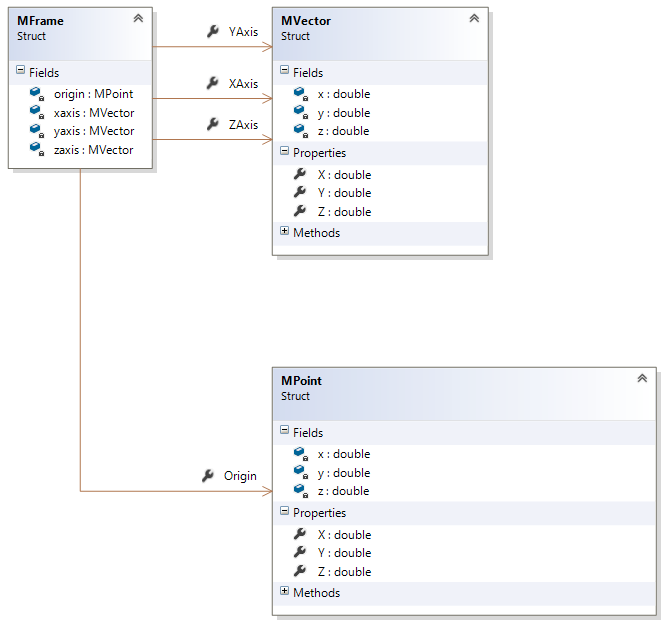
\includegraphics[width=0.8\textwidth]{mathlib.png}
	\captionof{figure}[]{Partial class diagram of \textit{Marsupilami.Math.dll}.}
	\label{fig:mathlib}
\end{figure}


\subsection{Structure of the algorithm}
The structure of the dynamic relaxation algorithm implemented in \emph{Marsupilami} is presented in \cref{alg:drmarsu}.

\IncMargin{2em}
\begin{figure}[p]
\begin{fullpage}
	\begin{algorithm}[H]
\footnotesize
\SetKwInOut{Input}{input}
\SetKwInOut{Output}{output}
\SetKwProg{Fn}{Function}{:}{}
\SetKwFunction{Solve}{Solve}
\SetKwFunction{Init}{Init}
\SetKwFunction{Run}{Run}
\SetKwFunction{Move}{Move}
\SetKwFunction{CalculateF}{CalcInternalForces}
\SetKwFunction{CalculateM}{CalcInternalMoments}
\SetKwFunction{CalculateA}{CalcAcceleration}
\SetKwFunction{CalculateV}{CalcVelocity}
\SetKwFunction{CalculateE}{CalcKEnergy}
\SetKwFunction{SumFM}{AggregateForcesAndMoments}
\SetKwFunction{SyncFM}{SynchronizeForcesAndMoments}
\SetKwFunction{SumM}{AggregateMasses}
\SetKwFunction{SyncM}{SynchronizeMasses}
\SetKwFunction{InterpX}{InterpolatePosition}
\SetKwFunction{InterpR}{InterpolatePosition}
\SetKwFunction{Reset}{Reset}

\SetKwData{Model}{model}
\SetKwData{Node}{node}
\SetKwData{Joint}{joint}
\SetKwData{Element}{element}
\SetKwData{CVG}{cvg}
\SetKwData{MAX}{maxIteration}

%\Input{A model to analyzed}
%\Output{An analyzed model}

% RUN
\Fn{\Run{}}{
\BlankLine
\ForEach(\tcc*[f]{$\vect{dx} = \vect{v_x}  dt$, $\vect{d\theta} = \vect{v_{\theta}}  dt$}){\Node in \Model}{
	\Move{$\vect{dx}, \vect{d\theta}$} \;
}
\BlankLine
\tcc{Elements calculate internal forces and moments}
\ForEach(){\Element in \Model}{
\CalculateF{$\vect{x}, \vect{d}_1,  \vect{d}_2,  \vect{d}_3$}
\tcc*[r]{$\vect{F}^{int}(\vect{x}, \vect{d}_1,  \vect{d}_2,  \vect{d}_3)$}

\CalculateM{$\vect{x}, \vect{d}_1,  \vect{d}_2,  \vect{d}_3$}
\tcc*[r]{$\vect{M}^{int}(\vect{x}, \vect{d}_1,  \vect{d}_2,  \vect{d}_3)$}
}
\BlankLine
\tcc{Joints coordinate the dynamic of several nodes}
\ForEach(){\Joint in \Model}{
\SumFM{} \;
\SumM{} \;
\SyncFM{} \;
\SyncM{} \;
}
\BlankLine
\tcc{Calculate translational kinetic energy}
\ForEach(){\Node in \Model}{
	\CalculateA{$m_x, \vect{F}$}
	\tcc*[f]{$\vect{a_x}(t) = \vect{R_x}/m_x$}
	
	\CalculateV{$\vect{a_x}, dt$}
	\tcc*[f]{$\vect{v_x}(t+\tfrac{dt}{2}) = \vect{v_x}(t-\tfrac{dt}{2}) + dt \vect{a_x}(t)$}
	
	\CalculateE{$\vect{v_x}$}
	\tcc*[f]{$E_x(t+\tfrac{dt}{2}) =  \tfrac{1}{2}\sum m_x \vect{v_x}^2(t+\tfrac{dt}{2})$}
}
\BlankLine
\tcc{Detect pic of kinetic energy}
\If{$E_x(t+\tfrac{dt}{2}) < E_x(t-\tfrac{dt}{2})$}{
	\InterpX{} \;
	\Reset{} \;
}

\BlankLine
\tcc{Calculate rotational kinetic energy}
\ForEach(){\Node in \Model}{
	\CalculateA{$m_{\theta}, \vect{M}$}
	\tcc*[f]{$\vect{a_{\theta}}(t) = \vect{R_x}/m_{\theta}$}
	
	\CalculateV{$\vect{a_{\theta}}, dt$}
	\tcc*[f]{$\vect{v_{\theta}}(t+\tfrac{dt}{2}) = \vect{v_{\theta}}(t-\tfrac{dt}{2}) + dt \vect{a_{\theta}}(t)$}
	
	\CalculateE{$\vect{v_{\theta}}$}
	\tcc*[f]{$E_{\theta} = \tfrac{1}{2}\sum m \vect{v_{\theta}}^2(t+\tfrac{dt}{2})$}
}
\BlankLine
\tcc{Detect pic of kinetic energy}
\If{$E_{\theta}(t+\tfrac{dt}{2})  < E_{\theta}(t-\tfrac{dt}{2})$}{
	\InterpR{} \;
	\Reset{} \;
}

}{\KwRet}
%\caption{Dynamic Relaxation algorithm as implemented in Marsupliami}
\captionof{algocf}[Dynamic Relaxation algorithm as implemented in \emph{Marsupilami}]{Dynamic Relaxation algorithm as implemented in \emph{Marsupilami}.}\label{algo_drmarsu}
\label{alg:drmarsu}
\end{algorithm}
\end{fullpage}
\end{figure}
\DecMargin{2em}


\subsection{Key aspects}
Discussions about implementing dynamic relaxation can be found in the reports from \citef{Olsson2012} and \citef{Poulsen2015}.

% \subsubsection{Language}
% Why C\# ?

\subsubsection{Code abstraction}
To develop a code with the right level of abstraction, it is advisable to refer to common \emph{design patterns} \cite{Bishop2008, Clune2012}.

%Modularité : evaluation courbure, schéma d'intégration, autorefine, autobreak, plasticity
%Design pattern
%\cite{Clune2012} : An object-oriented architecture for extensible structural design software
%\cite{Bishop2008} : design patterns

\subsubsection{Event driven}
Part of the solver implementation has been written to be \emph{event driven}.\footnote{\blockquote{The events-driven paradigm means that an object called an "event" is sent to the program whenever something happens, without that "something" having to be polled in regular intervals to discover whether it has happened. That "event" may be trapped by the program to perform some actions (i.e. a "handler") -- either synchronous or asynchronous.}} This allows to programmatically alter the solving process during its own execution. For some problems, this paradigm is very powerful and can succeed where more classic procedural or functional programming will fail. For instance this paradigm is currently used to implement auto-refinement of the element. It can be used to deal with breakable materials. In the future, it can be employed to add a level of user interactivity so the user can play with design parameters and see in quasi real-time the results, enhancing its design capabilities and reactivity.

%Events-driven vs asynchronous vs parallel.
%Evènement vs procédural
%\blockquote{The events-driven paradigm means that an object called an "event" is sent to the program whenever something happens, without that "something" having to be polled in regular intervals to discover whether it has happened. That "event" may be trapped by the program to perform some actions (i.e. a "handler") -- either synchronous or asynchronous.
%Therefore, handling of events can either be synchronous or asynchronous. JavaScript, for example, uses a synchronous eventing system.
%Asynchronous means that actions can happen independent of the current "main" execution stream. Mind you, it does NOT mean "parallel", or "different thread". An "asynchronous" action may actually run on the main thread, blocking the "main" execution stream in the meantime. So don't confuse "asynchronous" with "multi-threading".
%You may say that, technically speaking, an asynchronous operation automatically assumes eventing -- at least "completed", "faulted" or "aborted/cancelled" events (one or more of these) are sent to the instigator of the operation (or the underlying O/S itself) to signal that the operation has ceased. Thus, async is always event-driven, but not the other way round.
%}

\subsubsection{Serialization}
Serialization should be investigated to allow persistance of model. SQL vs. NoSQL solutions should be compared~: SQlite, Json, XML seem good options.

\subsection{Performance}
Software optimization is both a very active field of research and a nightmare for non specialists. It is virtually impossible to find good rules of thumb in the literature to orient critical implementation decisions. For instance a question that looks so simple as~: \textquote{Should I use a Struct of Arrays or and Array of Structs ?} ... is not so simple at all ; and the answer is generally \textquote{It depends ...}. And indeed, it depends on the coding language you chose, the coding skills you have to make the language talk to the processor in the way you want and not in the way you think it will. It also depends on complex hardware considerations. Optimizations can be made at all levels of abstraction of a software, from the highest level (algorithm) to the lowest level (assembly code).

To embrace the complexity of this problematic the reader is invited to refer to the excellent book \emph{Writing High-Performance .NET Code} \cite{Watson2014}.

\subsubsection{Know what things cost}
When it comes to software performance, the first stage should always be to measure what things cost (see \href{https://msdn.microsoft.com/en-us/library/ms973852.aspx}{know what things cost}).\footnote{\url{https://msdn.microsoft.com/en-us/library/ms973852.aspx}} Once the bottlenecks are identified,
then the optimization of the critical pieces of code can begin. To this end, two tools were employed during the development of \emph{Marsupilami} :
\begin{itemize}
\item Cost Model~: a very simple cost model was established to assign a performance rating to each base math routine, based on the number of arithmetic and trigonometric  operations it performes (see \cref{tab:costmodel}). This cost model was established through micro benchmarks with the \href{https://github.com/Microsoft/perfview}{BenchmarkDotNet} library.
\item Measure~: performance measurements were conducted on full analysis of several test cases with the library \href{https://github.com/Microsoft/perfview}{PerfView}.
\end{itemize}

\begin{table}[!b]
\center
	\ra{1.0}
	\begin{tabularx}{0.4\textwidth}{@{} X ccccc @{}}
		\toprule
		 	& add 	& sub 	& mul 	& div 	& sqrt \\
		\midrule
		cost	& 1 		& 1 		& 4 		& 10 		& 20	\\
		\bottomrule
	\end{tabularx}
	\label{tab:count}
	\vspace{10pt}
	\captionof{table}[Simple cost model for arithmetic operations]{Simple cost model for arithmetic operations.}
	\label{tab:costmodel}
\end{table}

\subsubsection{Algorithmic optimization}
The analyses made with PerfView showed that rotation and parallel transportation of frames are critical operations for the performance of the program. A thorough work was done to optimize all the costly math routines by using the minimal logic to perform the operations.

Further improvements might be achieved using polynomial representations of trigonometric functions but no time was left to dig seriously into this direction \cite{Trefethen2007,Chevillard2010}.\cite{Green2003}. The optimization of math routines and in particular trigonometric functions is a field of research to itself \cite{Green2003}.

\subsubsection{Vectorization}
\emph{Marsupilami} leverages the built-in capabilities offered by the .Net framework to parallelize some of the work. At the moment, the computation of the internal forces and moments of the elements is made inside a parallel loop. Still, a lot remains to be explored in this area~:
\begin{itemize}
\item Single Instruction Multiple Data (SIMD) instructions allow vectorization of arithmetic and trigonometric operations at the CPU level and can offer up to a x8 speed up.
\item Dynamic relaxation is very suitable for parallelization \cite{Topping1994}. New hardware capabilities such as multicore CPU or GPU cards with hundreds of cores can be leveraged to speed up the computation \cite{Rek2016,Liew2016}.
\end{itemize}
However, this technologies are relatively recent and still complex to implement as they require low level coding. They are note easily implementable from C\# and \emph{Marsupilami} does not rely on any of these technologies.

\subsubsection{Code abstraction}
\blockcquote[p.~155]{Watson2014}{In-depth performance optimization will often defy code abstractions.}

\subsection{Further guidelines}
This is a raw list of interesting ressources.
\subsubsection{Tips}

\begin{itemize}
\item abstract model
\item NLopt, Ipopt that have a C\# warper, accord-framework, alglib
\item Proprietary solver Knitro, Mosek
\item webAPI C\# Julia Javascript
\cite{Moulard2014} : Software Tools for Nonlinear Optimization
\end{itemize}

\href{https://neos-guide.org/}{Neos}
The NEOS Server is a free internet-based service for solving numerical optimization problems. It is able to take models specified in a variety of formats (including AMPL, GAMS and MPS) and pass them to a range of both free and commercial solvers (including Gurobi, CPLEX and Cbc). See here for the full list of solvers and input formats that NEOS supports.
https://github.com/odow/NEOS.jl
http://www.juliaopt.org/

\subsubsection{DifferentialEquations.jl}
(\href{http://docs.juliadiffeq.org/latest/index.html}{Manual} | \href{https://github.com/JuliaDiffEq}{GitHub})
Time integration, custom mass matrix, call back to implement kinetic damping, custom integrator

MathOptInterface.jl :

An abstraction layer for mathematical optimization solvers (\href{http://www.juliaopt.org/MathOptInterface.jl/latest/apimanual.html}{Manual} | \href{https://github.com/JuliaOpt/MathOptInterface.jl}{GitHub})
MathProgBase.jl :
This package provides high-level one-shot functions for linear and mixed-integer programming (linprog and mixintprog), as well as a solver-independent low-level interface for implementing advanced techniques that require efficiently solving a sequence of linear programming problems.
\url{http://mathprogbasejl.readthedocs.io/en/latest/index.html}

OOP vs structured programming : \url{https://softwareengineering.stackexchange.com/questions/125753/does-object-orientation-really-affect-algorithm-performance}
AoS vs OaS particle vs Collection of Particle.

\clearpage

\clearpage
\section{Test case}\label{sec=testcase}

The validation of the model is done through a comparison with the finite element solver \emph{Abaqus}. Several test cases have been studied to confirm that our model gives accurate results on typical problems where coupling between bending and torsion occurs.

\subsection{Constrained arch}\label{sec=testcase}

\subsubsection{Definition of the case}

In this test case, a straight slender beam ($L = \SI{10.0}{m}$) is bent into an arch-like shape (see \cref{fig:bench_arch}).\footnote{We previously employed this case in \cite{Lefevre2017}. A similar example was used by \citef{Bessini2017}.} The cross-section is rectangular ($\SI{4x6}{cm}$) and the bending occurs towards the strong inertia, provoking an out-of-plane displacement of the arch.\footnote{Note that if the arch had been bent against the weak inertia it would have remained planar.} The material axial and shear modulus are chosen to be $E=\SI{25}{GPa}$ and $G=\SI{10}{GPa}$ with a Poisson ratio of $\nu=0.25$.

The beam is supposed to be clamped at both ends, so that the material tangent $\vect{d}_3$ is forced to lie in the $xz$ plane, making an angle of magnitude $\pi/3$ with respect to the $x$ axis, and so that the second material axis $\vect{d}_2$ is collinear to the $y$ axis. The distance between the ends is set to $\SI{2.0}{m}$.
\begin{figure}[!h]
     	\centering
	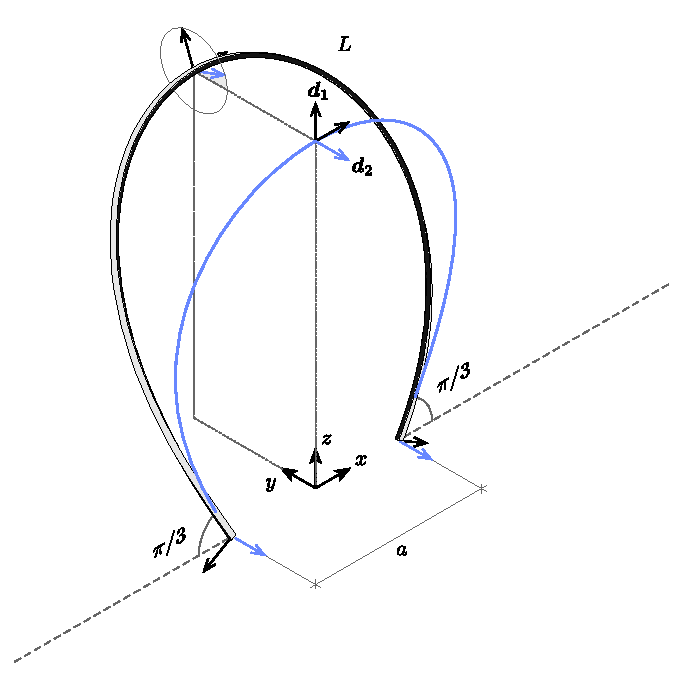
\includegraphics[width=0.8\textwidth]{bench_A.pdf}
	\captionof{figure}[Test case of a constrained arch]{Test case of a constrained arch.}
	\label{fig:bench_arch}
\end{figure}

\subsubsection{Results}

The problem is solved with \emph{Marsupilami} and \emph{Abaqus} for different values of the discretization, respectively $6$, $12$, $24$, $48$ and $96$ elements or segments.\footnote{In Abaqus the beam element is set to B31.}

The results of the computations are summarized in tables where the black color stands for \emph{Abaqus} and the blue color stands for \emph{Marsupilami}. Each studied parameter owns two lines in a table~: the first line is populated with the value of the parameter while the second line is populated with the relative error from the target result. The target result is always chosen to be the value from \emph{Abaqus} with the finest discretization ($96$ elements).

For instance, the $y$ component of the apex value for a beam discretized with $6$ elements is $1.455$ with \emph{Marsupilami} and $1.643$ for \emph{Abaqus} (see \cref{tab:resA_geo}). The target value is $1.459$. Thus, the relative errors are respectively given by $1.455/1.459 -1 = -0.3\%$ and $1.643/1.459 -1 = 12.6\%$.

The first table compares the discrete and smooth lengths of the model, where the smooth length is interpolated from the discrete model. It also gives the coordinates ($x$, $y$, $z$) of the apex point of the arch (see \cref{tab:resA_geo}). The second table compares the axial ($N$) and shear ($F_1$, $F_2$) forces in the beam at the start ($s=0$), at the apex ($s=L/2$) and at the end ($s=L$) of the beam (see \cref{tab:resA_force}). The third table compares the twisting ($Q$) and bending ($M_1$, $M_2$) moments in the beam at the start($s=0$), at the apex ($s=L/2$) and at the end ($s=L$) of the beam (see \cref{tab:resA_moment}).

Additionally, we provide full internal force diagrams for the finest discretization with $96$ elements (see \cref{fig:bench_arch_diagram}). The results from \emph{Abaqus} are plotted as a solid grey color while the results from \emph{Marsupilami} are plotted as a bold dashed blue line. Note that the results are normalized.

\begin{figure}[p]
\begin{fullpage}
     	\centering
	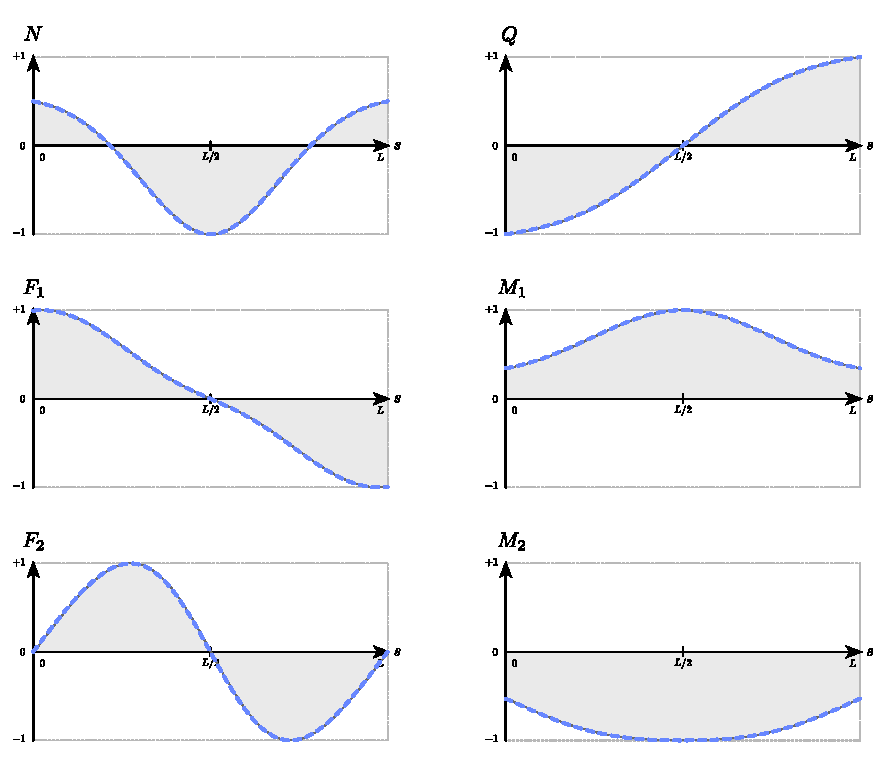
\includegraphics[width=0.9\textwidth]{bench_arch_diagram.pdf}
	\captionof{figure}[Comparison of normalized force diagrams]{Comparison of normalized normalized force diagrams for the finest discretization ($n_{el}=96$ | Marsupilami~: blue | Abaqus : grey).}
	\label{fig:bench_arch_diagram}
\end{fullpage}
\end{figure}

\begin{figure}[p]
\begin{fullpage}
\centering
\ra{1.0}
%\begin{tabu} to 0.75\linewidth{@{}X[1.5] X[1.5] *5{X[1,r,b]}@{}}
\begin{tabularx}{0.75\textwidth}{@{} XX rrrrr@{}}
\toprule
& & \multicolumn{5}{c}{number of elements / segments} \\\cmidrule{3-7}
&  &  6 & 12 & 24 & 48 & 96 \\
\midrule
\multirow{8}{*}{Length}&\multirow{4}{*}{smooth}&{\color{Tblue}\normalsize10.262}&{\color{Tblue}\normalsize10.065}&{\color{Tblue}\normalsize10.016}&{\color{Tblue}\normalsize10.004}&{\color{Tblue}\normalsize10.001}\\
&&{\color{Tblue}\scriptsize2.6\%}&{\color{Tblue}\scriptsize0.6\%}&{\color{Tblue}\scriptsize0.2\%}&{\color{Tblue}\scriptsize0.0\%}&{\color{Tblue}\scriptsize0.0\%}\\
&&{\color{black}\normalsize10.261}&{\color{black}\normalsize10.065}&{\color{black}\normalsize10.016}&{\color{black}\normalsize10.004}&{\color{black}\normalsize10.001}\\
&&{\color{black}\scriptsize2.6\%}&{\color{black}\scriptsize0.6\%}&{\color{black}\scriptsize0.2\%}&{\color{black}\scriptsize0.0\%}&{\color{black}\scriptsize0.0\%}\\\cmidrule[0.5\cmidrulewidth]{2-7}
&\multirow{4}{*}{discrete}&{\color{Tblue}\normalsize10.000}&{\color{Tblue}\normalsize10.000}&{\color{Tblue}\normalsize10.000}&{\color{Tblue}\normalsize10.000}&{\color{Tblue}\normalsize10.000}\\
&&{\color{Tblue}\scriptsize0.0\%}&{\color{Tblue}\scriptsize0.0\%}&{\color{Tblue}\scriptsize0.0\%}&{\color{Tblue}\scriptsize0.0\%}&{\color{Tblue}\scriptsize0.0\%}\\
&&{\color{black}\normalsize10.000}&{\color{black}\normalsize10.000}&{\color{black}\normalsize10.000}&{\color{black}\normalsize10.000}&{\color{black}\normalsize10.000}\\
&&{\color{black}\scriptsize0.0\%}&{\color{black}\scriptsize0.0\%}&{\color{black}\scriptsize0.0\%}&{\color{black}\scriptsize0.0\%}&{\color{black}\scriptsize0.0\%}\\\midrule
\multirow{12}{*}{Apex}  &\multirow{4}{*}{$x$}&{\color{Tblue}\normalsize-0.001}&{\color{Tblue}\normalsize0.000}&{\color{Tblue}\normalsize0.000}&{\color{Tblue}\normalsize0.000}&{\color{Tblue}\normalsize0.000}\\
&&{\color{Tblue}\scriptsize-}&{\color{Tblue}\scriptsize-}&{\color{Tblue}\scriptsize-}&{\color{Tblue}\scriptsize-}&{\color{Tblue}\scriptsize-}\\
&&{\color{black}\normalsize0.000}&{\color{black}\normalsize0.000}&{\color{black}\normalsize0.000}&{\color{black}\normalsize0.000}&{\color{black}\normalsize0.000}\\
&&{\color{black}\scriptsize-}&{\color{black}\scriptsize-}&{\color{black}\scriptsize-}&{\color{black}\scriptsize-}&{\color{black}\scriptsize-}\\\cmidrule[0.5\cmidrulewidth]{2-7}
&\multirow{4}{*}{$y$}&{\color{Tblue}\normalsize1.455}&{\color{Tblue}\normalsize1.453}&{\color{Tblue}\normalsize1.457}&{\color{Tblue}\normalsize1.458}&{\color{Tblue}\normalsize1.458}\\
&&{\color{Tblue}\scriptsize-0.3\%}&{\color{Tblue}\scriptsize-0.4\%}&{\color{Tblue}\scriptsize-0.1\%}&{\color{Tblue}\scriptsize-0.1\%}&{\color{Tblue}\scriptsize-0.1\%}\\
&&{\color{black}\normalsize1.643}&{\color{black}\normalsize1.506}&{\color{black}\normalsize1.471}&{\color{black}\normalsize1.462}&{\color{black}\normalsize1.459}\\
&&{\color{black}\scriptsize12.6\%}&{\color{black}\scriptsize3.2\%}&{\color{black}\scriptsize0.8\%}&{\color{black}\scriptsize0.2\%}&{\color{black}\scriptsize0.0\%}\\\cmidrule[0.5\cmidrulewidth]{2-7}
&\multirow{4}{*}{$z$}&{\color{Tblue}\normalsize3.665}&{\color{Tblue}\normalsize3.615}&{\color{Tblue}\normalsize3.601}&{\color{Tblue}\normalsize3.598}&{\color{Tblue}\normalsize3.597}\\
&&{\color{Tblue}\scriptsize1.9\%}&{\color{Tblue}\scriptsize0.5\%}&{\color{Tblue}\scriptsize0.1\%}&{\color{Tblue}\scriptsize0.0\%}&{\color{Tblue}\scriptsize0.0\%}\\
&&{\color{black}\normalsize3.593}&{\color{black}\normalsize3.595}&{\color{black}\normalsize3.596}&{\color{black}\normalsize3.596}&{\color{black}\normalsize3.597}\\
&&{\color{black}\scriptsize-0.1\%}&{\color{black}\scriptsize-0.1\%}&{\color{black}\scriptsize0.0\%}&{\color{black}\scriptsize0.0\%}&{\color{black}\scriptsize0.0\%}\\
\bottomrule
\end{tabularx}
\captionof{table}[Geometric parameters for the arch test case]{Geometric parameters for the arch test case (Marsupilami~: blue | Abaqus : black).}
\label{tab:resA_geo}
\end{fullpage}
\end{figure}

\subsubsection{Discussion}

The results show a very good correlation between our model and the results from \emph{Abaqus}, even for coarse discretizations. With only $24$ elements, the maximum relative error of our model is $0.1\%$ for the position of the apex and $1.4\%$ for the internal force and moment at critical points.

The superposition of the internal force diagrams obtained for the finest discretization show a very accurate match between our model and the results from \emph{Abaqus} (see \cref{fig:bench_arch_diagram}).

\begin{figure}[p]
	\centering
	\begin{fullpage}
\ra{1.0}
%\begin{tabu} to 0.75\linewidth{@{}X[1cm,c,m] X[0.5cm,c,m] *5{X[1.0cm,r,b]}<{\strut}@{}}
\begin{tabularx}{0.6\textwidth}{@{} XX rrrrr@{}}
\toprule
& & \multicolumn{5}{c}{number of elements / segments} \\ \cmidrule{3-7}
&  &  6 & 12 & 24 & 48 & 96 \\
\midrule
\multirow{12}{*}{$N$}&\multirow{4}{*}{$0$}&{\color{Tblue}\normalsize 179}&{\color{Tblue}\normalsize 275}&{\color{Tblue}\normalsize 302}&{\color{Tblue}\normalsize 308}&{\color{Tblue}\normalsize 310}\\
&&{\color{Tblue}\scriptsize-41.4\%}&{\color{Tblue}\scriptsize-10.1\%}&{\color{Tblue}\scriptsize-1.4\%}&{\color{Tblue}\scriptsize0.8\%}&{\color{Tblue}\scriptsize1.3\%}\\
&&{\color{black}\normalsize 311}&{\color{black}\normalsize 304}&{\color{black}\normalsize 305}&{\color{black}\normalsize 307}&{\color{black}\normalsize 306}\\
&&{\color{black}\scriptsize1.7\%}&{\color{black}\scriptsize-0.6\%}&{\color{black}\scriptsize-0.5\%}&{\color{black}\scriptsize0.2\%}&{\color{black}\scriptsize0.0\%}\\\cmidrule[0.5\cmidrulewidth]{2-7}
&\multirow{4}{*}{$L/2$}&{\color{Tblue}\normalsize- 475}&{\color{Tblue}\normalsize- 585}&{\color{Tblue}\normalsize- 612}&{\color{Tblue}\normalsize- 619}&{\color{Tblue}\normalsize- 620}\\
&&{\color{Tblue}\scriptsize-23.6\%}&{\color{Tblue}\scriptsize-5.9\%}&{\color{Tblue}\scriptsize-1.5\%}&{\color{Tblue}\scriptsize-0.4\%}&{\color{Tblue}\scriptsize-0.2\%}\\
&&{\color{black}\normalsize- 669}&{\color{black}\normalsize- 633}&{\color{black}\normalsize- 624}&{\color{black}\normalsize- 622}&{\color{black}\normalsize- 622}\\
&&{\color{black}\scriptsize7.7\%}&{\color{black}\scriptsize1.9\%}&{\color{black}\scriptsize0.4\%}&{\color{black}\scriptsize0.0\%}&{\color{black}\scriptsize0.0\%}\\\cmidrule[0.5\cmidrulewidth]{2-7}
&\multirow{4}{*}{$L$}&{\color{Tblue}\normalsize 181}&{\color{Tblue}\normalsize 275}&{\color{Tblue}\normalsize 302}&{\color{Tblue}\normalsize 308}&{\color{Tblue}\normalsize 310}\\
&&{\color{Tblue}\scriptsize-40.8\%}&{\color{Tblue}\scriptsize-10.1\%}&{\color{Tblue}\scriptsize-1.4\%}&{\color{Tblue}\scriptsize0.8\%}&{\color{Tblue}\scriptsize1.3\%}\\
&&{\color{black}\normalsize 311}&{\color{black}\normalsize 304}&{\color{black}\normalsize 305}&{\color{black}\normalsize 307}&{\color{black}\normalsize 306}\\
&&{\color{black}\scriptsize1.7\%}&{\color{black}\scriptsize-0.6\%}&{\color{black}\scriptsize-0.5\%}&{\color{black}\scriptsize0.2\%}&{\color{black}\scriptsize0.0\%}\\\midrule
\multirow{12}{*}{$F1$}&\multirow{4}{*}{$0$}&{\color{Tblue}\normalsize 434}&{\color{Tblue}\normalsize 515}&{\color{Tblue}\normalsize 532}&{\color{Tblue}\normalsize 537}&{\color{Tblue}\normalsize 538}\\
&&{\color{Tblue}\scriptsize-19.7\%}&{\color{Tblue}\scriptsize-4.7\%}&{\color{Tblue}\scriptsize-1.4\%}&{\color{Tblue}\scriptsize-0.6\%}&{\color{Tblue}\scriptsize-0.5\%}\\
&&{\color{black}\normalsize 634}&{\color{black}\normalsize 567}&{\color{black}\normalsize 548}&{\color{black}\normalsize 542}&{\color{black}\normalsize 540}\\
&&{\color{black}\scriptsize17.3\%}&{\color{black}\scriptsize4.9\%}&{\color{black}\scriptsize1.4\%}&{\color{black}\scriptsize0.3\%}&{\color{black}\scriptsize0.0\%}\\\cmidrule[0.5\cmidrulewidth]{2-7}
&\multirow{4}{*}{$L/2$}&{\color{Tblue}\normalsize 2}&{\color{Tblue}\normalsize 0}&{\color{Tblue}\normalsize 0}&{\color{Tblue}\normalsize 0}&{\color{Tblue}\normalsize 0}\\
&&{\color{Tblue}\scriptsize-}&{\color{Tblue}\scriptsize-}&{\color{Tblue}\scriptsize-}&{\color{Tblue}\scriptsize-}&{\color{Tblue}\scriptsize-}\\
&&{\color{black}\normalsize 0}&{\color{black}\normalsize 0}&{\color{black}\normalsize 0}&{\color{black}\normalsize 0}&{\color{black}\normalsize 0}\\
&&{\color{black}\scriptsize-}&{\color{black}\scriptsize-}&{\color{black}\scriptsize-}&{\color{black}\scriptsize-}&{\color{black}\scriptsize-}\\\cmidrule[0.5\cmidrulewidth]{2-7}
&\multirow{4}{*}{$L$}&{\color{Tblue}\normalsize- 432}&{\color{Tblue}\normalsize- 515}&{\color{Tblue}\normalsize- 532}&{\color{Tblue}\normalsize- 537}&{\color{Tblue}\normalsize- 538}\\
&&{\color{Tblue}\scriptsize-19.9\%}&{\color{Tblue}\scriptsize-4.7\%}&{\color{Tblue}\scriptsize-1.4\%}&{\color{Tblue}\scriptsize-0.6\%}&{\color{Tblue}\scriptsize-0.5\%}\\
&&{\color{black}\normalsize- 634}&{\color{black}\normalsize- 567}&{\color{black}\normalsize- 548}&{\color{black}\normalsize- 542}&{\color{black}\normalsize- 540}\\
&&{\color{black}\scriptsize17.3\%}&{\color{black}\scriptsize4.9\%}&{\color{black}\scriptsize1.4\%}&{\color{black}\scriptsize0.3\%}&{\color{black}\scriptsize0.0\%}\\\midrule
\multirow{12}{*}{$F2$}&\multirow{4}{*}{$0$}&{\color{Tblue}\normalsize 73}&{\color{Tblue}\normalsize 29}&{\color{Tblue}\normalsize 8}&{\color{Tblue}\normalsize 2}&{\color{Tblue}\normalsize 1}\\
&&{\color{Tblue}\scriptsize-}&{\color{Tblue}\scriptsize-}&{\color{Tblue}\scriptsize-}&{\color{Tblue}\scriptsize-}&{\color{Tblue}\scriptsize-}\\
&&{\color{black}\normalsize 306}&{\color{black}\normalsize 129}&{\color{black}\normalsize 61}&{\color{black}\normalsize 30}&{\color{black}\normalsize 15}\\
&&{\color{black}\scriptsize-}&{\color{black}\scriptsize-}&{\color{black}\scriptsize-}&{\color{black}\scriptsize-}&{\color{black}\scriptsize-}\\\cmidrule[0.5\cmidrulewidth]{2-7}
&\multirow{4}{*}{$L/2$}&{\color{Tblue}\normalsize 0}&{\color{Tblue}\normalsize 0}&{\color{Tblue}\normalsize 0}&{\color{Tblue}\normalsize 0}&{\color{Tblue}\normalsize 0}\\
&&{\color{Tblue}\scriptsize-}&{\color{Tblue}\scriptsize-}&{\color{Tblue}\scriptsize-}&{\color{Tblue}\scriptsize-}&{\color{Tblue}\scriptsize-}\\
&&{\color{black}\normalsize 0}&{\color{black}\normalsize 0}&{\color{black}\normalsize 0}&{\color{black}\normalsize 0}&{\color{black}\normalsize 0}\\
&&{\color{black}\scriptsize-}&{\color{black}\scriptsize-}&{\color{black}\scriptsize-}&{\color{black}\scriptsize-}&{\color{black}\scriptsize-}\\\cmidrule[0.5\cmidrulewidth]{2-7}
&\multirow{4}{*}{$L$}&{\color{Tblue}\normalsize- 66}&{\color{Tblue}\normalsize- 29}&{\color{Tblue}\normalsize- 8}&{\color{Tblue}\normalsize- 2}&{\color{Tblue}\normalsize- 1}\\
&&{\color{Tblue}\scriptsize-}&{\color{Tblue}\scriptsize-}&{\color{Tblue}\scriptsize-}&{\color{Tblue}\scriptsize-}&{\color{Tblue}\scriptsize-}\\
&&{\color{black}\normalsize- 306}&{\color{black}\normalsize- 129}&{\color{black}\normalsize- 61}&{\color{black}\normalsize- 30}&{\color{black}\normalsize- 15}\\
&&{\color{black}\scriptsize-}&{\color{black}\scriptsize-}&{\color{black}\scriptsize-}&{\color{black}\scriptsize-}&{\color{black}\scriptsize-}\\
\bottomrule
\end{tabularx}
\captionof{table}[Internal forces for the arch test case]{Internal forces for the arch test case (Marsupilami~: blue | Abaqus : black).}
\label{tab:resA_force}
	\end{fullpage}
\end{figure}
\begin{figure}[p]
	\centering
	\begin{fullpage}
\ra{1.0}
%\begin{tabu} to 0.75\linewidth{@{}X[1cm,c,m] X[0.5cm,c,m] *5{X[1.0cm,r,b]}<{\strut}@{}}
\begin{tabularx}{0.65\textwidth}{@{} XX rrrrr@{}}
\toprule
& & \multicolumn{5}{c}{number of elements / segments} \\ \cmidrule{3-7}
&  &  6 & 12 & 24 & 48 & 96 \\
\midrule
\multirow{12}{*}{$Q$}&\multirow{4}{*}{$0$}&{\color{Tblue}\normalsize-3 092}&{\color{Tblue}\normalsize-3 009}&{\color{Tblue}\normalsize-2 989}&{\color{Tblue}\normalsize-2 985}&{\color{Tblue}\normalsize-2 984}\\
&&{\color{Tblue}\scriptsize3.9\%}&{\color{Tblue}\scriptsize1.1\%}&{\color{Tblue}\scriptsize0.4\%}&{\color{Tblue}\scriptsize0.3\%}&{\color{Tblue}\scriptsize0.3\%}\\
&&{\color{black}\normalsize-2 731}&{\color{black}\normalsize-2 885}&{\color{black}\normalsize-2 942}&{\color{black}\normalsize-2 965}&{\color{black}\normalsize-2 976}\\
&&{\color{black}\scriptsize-8.2\%}&{\color{black}\scriptsize-3.1\%}&{\color{black}\scriptsize-1.1\%}&{\color{black}\scriptsize-0.4\%}&{\color{black}\scriptsize0.0\%}\\\cmidrule[0.5\cmidrulewidth]{2-7}
&\multirow{4}{*}{$L/2$}&{\color{Tblue}\normalsize 0}&{\color{Tblue}\normalsize 0}&{\color{Tblue}\normalsize 0}&{\color{Tblue}\normalsize 0}&{\color{Tblue}\normalsize 0}\\
&&{\color{Tblue}\scriptsize-}&{\color{Tblue}\scriptsize-}&{\color{Tblue}\scriptsize-}&{\color{Tblue}\scriptsize-}&{\color{Tblue}\scriptsize-}\\
&&{\color{black}\normalsize 0}&{\color{black}\normalsize 0}&{\color{black}\normalsize 0}&{\color{black}\normalsize 0}&{\color{black}\normalsize 0}\\
&&{\color{black}\scriptsize-}&{\color{black}\scriptsize-}&{\color{black}\scriptsize-}&{\color{black}\scriptsize-}&{\color{black}\scriptsize-}\\\cmidrule[0.5\cmidrulewidth]{2-7}
&\multirow{4}{*}{$L$}&{\color{Tblue}\normalsize3 095}&{\color{Tblue}\normalsize3 009}&{\color{Tblue}\normalsize2 989}&{\color{Tblue}\normalsize2 985}&{\color{Tblue}\normalsize2 984}\\
&&{\color{Tblue}\scriptsize4.0\%}&{\color{Tblue}\scriptsize1.1\%}&{\color{Tblue}\scriptsize0.4\%}&{\color{Tblue}\scriptsize0.3\%}&{\color{Tblue}\scriptsize0.3\%}\\
&&{\color{black}\normalsize2 731}&{\color{black}\normalsize2 885}&{\color{black}\normalsize2 942}&{\color{black}\normalsize2 965}&{\color{black}\normalsize2 976}\\
&&{\color{black}\scriptsize-8.2\%}&{\color{black}\scriptsize-3.1\%}&{\color{black}\scriptsize-1.1\%}&{\color{black}\scriptsize-0.4\%}&{\color{black}\scriptsize0.0\%}\\\midrule
\multirow{12}{*}{$M1$}&\multirow{4}{*}{$0$}&{\color{Tblue}\normalsize1 548}&{\color{Tblue}\normalsize1 669}&{\color{Tblue}\normalsize1 709}&{\color{Tblue}\normalsize1 719}&{\color{Tblue}\normalsize1 721}\\
&&{\color{Tblue}\scriptsize-11.1\%}&{\color{Tblue}\scriptsize-4.1\%}&{\color{Tblue}\scriptsize-1.8\%}&{\color{Tblue}\scriptsize-1.2\%}&{\color{Tblue}\scriptsize-1.1\%}\\
&&{\color{black}\normalsize1 934}&{\color{black}\normalsize1 863}&{\color{black}\normalsize1 795}&{\color{black}\normalsize1 759}&{\color{black}\normalsize1 740}\\
&&{\color{black}\scriptsize11.1\%}&{\color{black}\scriptsize7.1\%}&{\color{black}\scriptsize3.2\%}&{\color{black}\scriptsize1.1\%}&{\color{black}\scriptsize0.0\%}\\\cmidrule[0.5\cmidrulewidth]{2-7}
&\multirow{4}{*}{$L/2$}&{\color{Tblue}\normalsize4 577}&{\color{Tblue}\normalsize4 881}&{\color{Tblue}\normalsize4 964}&{\color{Tblue}\normalsize4 986}&{\color{Tblue}\normalsize4 991}\\
&&{\color{Tblue}\scriptsize-8.3\%}&{\color{Tblue}\scriptsize-2.2\%}&{\color{Tblue}\scriptsize-0.6\%}&{\color{Tblue}\scriptsize-0.1\%}&{\color{Tblue}\scriptsize0.0\%}\\
&&{\color{black}\normalsize5 106}&{\color{black}\normalsize5 017}&{\color{black}\normalsize4 998}&{\color{black}\normalsize4 994}&{\color{black}\normalsize4 992}\\
&&{\color{black}\scriptsize2.3\%}&{\color{black}\scriptsize0.5\%}&{\color{black}\scriptsize0.1\%}&{\color{black}\scriptsize0.0\%}&{\color{black}\scriptsize0.0\%}\\\cmidrule[0.5\cmidrulewidth]{2-7}
&\multirow{4}{*}{$L$}&{\color{Tblue}\normalsize1 556}&{\color{Tblue}\normalsize1 669}&{\color{Tblue}\normalsize1 709}&{\color{Tblue}\normalsize1 719}&{\color{Tblue}\normalsize1 721}\\
&&{\color{Tblue}\scriptsize-10.6\%}&{\color{Tblue}\scriptsize-4.1\%}&{\color{Tblue}\scriptsize-1.8\%}&{\color{Tblue}\scriptsize-1.2\%}&{\color{Tblue}\scriptsize-1.1\%}\\
&&{\color{black}\normalsize1 934}&{\color{black}\normalsize1 863}&{\color{black}\normalsize1 795}&{\color{black}\normalsize1 759}&{\color{black}\normalsize1 740}\\
&&{\color{black}\scriptsize11.1\%}&{\color{black}\scriptsize7.1\%}&{\color{black}\scriptsize3.2\%}&{\color{black}\scriptsize1.1\%}&{\color{black}\scriptsize0.0\%}\\\midrule
\multirow{12}{*}{$M2$}&\multirow{4}{*}{$0$}&{\color{Tblue}\normalsize-2 014}&{\color{Tblue}\normalsize-1 597}&{\color{Tblue}\normalsize-1 490}&{\color{Tblue}\normalsize-1 464}&{\color{Tblue}\normalsize-1 458}\\
&&{\color{Tblue}\scriptsize38.7\%}&{\color{Tblue}\scriptsize9.9\%}&{\color{Tblue}\scriptsize2.6\%}&{\color{Tblue}\scriptsize0.8\%}&{\color{Tblue}\scriptsize0.4\%}\\
&&{\color{black}\normalsize-1 231}&{\color{black}\normalsize-1 378}&{\color{black}\normalsize-1 430}&{\color{black}\normalsize-1 447}&{\color{black}\normalsize-1 453}\\
&&{\color{black}\scriptsize-15.3\%}&{\color{black}\scriptsize-5.2\%}&{\color{black}\scriptsize-1.6\%}&{\color{black}\scriptsize-0.4\%}&{\color{black}\scriptsize0.0\%}\\\cmidrule[0.5\cmidrulewidth]{2-7}
&\multirow{4}{*}{$L/2$}&{\color{Tblue}\normalsize-2 918}&{\color{Tblue}\normalsize-2 791}&{\color{Tblue}\normalsize-2 766}&{\color{Tblue}\normalsize-2 761}&{\color{Tblue}\normalsize-2 760}\\
&&{\color{Tblue}\scriptsize5.6\%}&{\color{Tblue}\scriptsize1.0\%}&{\color{Tblue}\scriptsize0.1\%}&{\color{Tblue}\scriptsize0.0\%}&{\color{Tblue}\scriptsize-0.1\%}\\
&&{\color{black}\normalsize-3 217}&{\color{black}\normalsize-2 868}&{\color{black}\normalsize-2 788}&{\color{black}\normalsize-2 768}&{\color{black}\normalsize-2 763}\\
&&{\color{black}\scriptsize16.5\%}&{\color{black}\scriptsize3.8\%}&{\color{black}\scriptsize0.9\%}&{\color{black}\scriptsize0.2\%}&{\color{black}\scriptsize0.0\%}\\\cmidrule[0.5\cmidrulewidth]{2-7}
&\multirow{4}{*}{$L$}&{\color{Tblue}\normalsize-2 015}&{\color{Tblue}\normalsize-1 597}&{\color{Tblue}\normalsize-1 490}&{\color{Tblue}\normalsize-1 464}&{\color{Tblue}\normalsize-1 458}\\
&&{\color{Tblue}\scriptsize38.7\%}&{\color{Tblue}\scriptsize10.0\%}&{\color{Tblue}\scriptsize2.6\%}&{\color{Tblue}\scriptsize0.8\%}&{\color{Tblue}\scriptsize0.4\%}\\
&&{\color{black}\normalsize-1 231}&{\color{black}\normalsize-1 378}&{\color{black}\normalsize-1 430}&{\color{black}\normalsize-1 447}&{\color{black}\normalsize-1 453}\\
&&{\color{black}\scriptsize-15.3\%}&{\color{black}\scriptsize-5.2\%}&{\color{black}\scriptsize-1.6\%}&{\color{black}\scriptsize-0.4\%}&{\color{black}\scriptsize0.0\%}\\\bottomrule
\end{tabularx}
\captionof{table}[Internal moments for the arch test case]{Internal moments for the arch test case (Marsupilami~: blue | Abaqus : black).}
\label{tab:resA_moment}
	\end{fullpage}
\end{figure}
\clearpage
\subsection{Cantilever beam}
To be added. Cantilever beam with punctual force and moment load to show how our model is able to render discontinuities accurately.

\section{Conclusion}

In this chapter, we have combined our relexions on the notion of discrete curvature (see \cref{chp=curve}) and the previous smooth beam model obtained from the dynamical equations of Kirchhoff (see \cref{chp=kirchhoff}). This led us to build a new discrete beam element with 4 degrees of freedom and 3 nodes, as opposed to 2 for the previous model. We have shown that this element naturally deals with the issue of external actions and fits perfectly into the conceptual framework of dynamic relaxation~; itself based on the fundamental principle of dynamics. The section and material properties of the element are assumed to be uniform over the length of the element. It can account for axial, bending and torsion behaviours of the beam, in the framework of Kirchhoff's theory, for sections whose torsional center coincides with the center of mass. It can undergo concentrated actions at its extremities and uniform distributed actions in the current part. The internal forces are therefore continuous along the length of the element but can undergo jumps at its ends. We also presented how free, rigid or elastic support conditions can be implemented in the model.

Finally, we have briefly introduced \emph{Marsupilami}, the computation code that we have developed and that implements this new element. It takes the form of a standalone \Csharp{} API. This API has been partially integrated into a \grasshopper{} component library intended as a graphical interface. Numerous options have been explored regarding the code architecture to birng new possibilities, notably thanks to the use of events (automatic mesh refinement, following force, parallelization of calculations, user interaction, \telp{}). The code tries to make the best of the abstractions proposed by the language \Csharp{} to marry different types of elements, conditions of support and even of nodes according to their number of degrees of freedom (3, 4 or 6). We were able to validate the accuracy of our new element by comparing the results of \emph{Marsupilami} with those of the software \emph{Abaqus} -- a reference in the field -- on various test cases. Performed on single beams, this validation work must be continued on complete structures. However, at the moment \emph{Marsupilami} is not a real software that could be used in a production context. In its current state, it is a proof of concept, which deserves a serious development effort to achieve a first stable reslease transferable to other users.